% Harbor Journal Paper
\documentclass[acmtecs,acmnow,a4paper]{acmtrans2m}
\usepackage{graphicx,amsmath,subfigure}

\newtheorem{theorem}{Theorem}[section]
\newtheorem{conjecture}[theorem]{Conjecture}
\newtheorem{corollary}[theorem]{Corollary}
\newtheorem{proposition}[theorem]{Proposition}
\newtheorem{lemma}[theorem]{Lemma}
\newdef{definition}[theorem]{Definition}
\newdef{remark}[theorem]{Remark}


           
\markboth{...}{...}

\title{Memory Protection in Resource Constrained Sensor Nodes}
            
\author{Ram Kumar, Akhilesh Singhania, Eddie Kohler, Mani Srivastava}
            
\begin{abstract} 
%==============================================================
% ABSTRACT
%==============================================================
\noindent
Many embedded systems contain resource constrained microcontrollers where applications, operating system components and device drivers reside within a single address space with no form of memory protection.
%
Programming errors in one application can easily corrupt the state of the operating system and other applications on the microcontroller.
%
In this paper we propose a system that provides memory protection in tiny embedded processors\footnote{8, 16 and 32-bit microcontrollers with limited resources}.
%
Our system consists of a software run-time working with minimal low-cost architectural extensions to the processor core that prevents corruption of state by buggy applications.
%
We restrict memory accesses and control flow of applications to \textit{protection domains} within the address space.
%
The software run-time consists of a \textit{Memory map}: a flexible and efficient data structure that records ownership and layout information of the entire address space.
%
Memory map checks are done for \texttt{store} instructions by hardware accelerators that significantly improve the performance of our system.
%
We preserve control flow integrity by maintaining a \textit{Safe stack} that stores return addresses in a protected memory region.
%
Cross domain function calls are redirected through a software based jump table.
%Domain switches within a single address space is done with the help of a cross domain linker tool that generates a software jump table.
%
Enhancements to the microcontroller \texttt{call} and \texttt{return} instructions use the jump table to track the current active domain.
%
We have implemented our scheme on a VHDL model of ATMEGA103 microcontroller.
%
Our evaluations show that embedded applications can enjoy the benefits of memory protection with minimal impact on performance and a modest increase in the area of the microcontroller.

\end{abstract}
            


\category{C.3}{Special Purpose and Application-Based Systems}{Real-time and embedded systems}
            
\terms{Performance, Design, Reliability} 
            
\keywords{Software Fault Isolation, Memory Protection}
            
\begin{document}
            
\begin{bottomstuff} 
...
\end{bottomstuff}
            
\maketitle


%%%%%%%%%%%%%%%%%%%%
% INTRODUCTION
%%%%%%%%%%%%%%%%%%%%
\section{Introduction}
\label{sec:introduction}
%
This paper explores the challenges in providing fault isolation
through memory protection on resource constrained embedded systems
such as sensor nodes.
%
%Sensor networks have promise for many industrial, commercial, and
%medical applications.
%
%For example, CodeBlue~\cite{welsh04codeblue} is a prototype medical
%sensor network platform for expediting triage during disaster
%response.
%
%A network of 4000 sensors deployed by Intel in a
%semiconductor fabrication plant performs predictive maintenance of
%machinery in service~\cite{intel05fabapp}.
%
%The Zigbee consortium~\cite{zigbee} seeks to equip lighting and
%HVAC controllers with wireless radios, enabling intelligent building
%automation and security services.
%
%These 
Current and upcoming sensor network deployments require high
availability infrastructure with the ability to support multiple users.
%
%
Unexpected system failures could cause problems ranging from financial
impacts to loss of life.
%
Current software technology is grossly inadequate to run such long
term deployments.
%
Bugs in any part of the software can easily bring down an entire network.
%
In particular, memory corruption due to buggy applications can crash or
freeze sensor nodes or corrupt sensed data.
%
We argue that memory protection is a vital enabling technology for
creating reliable and long-lasting sensor network software systems.
%

Sensor software is quite complex, supporting 
%
many sensor types, multiple distributed
middleware services, dynamic code updates, and concurrent applications.
%
Programmers must deal with severe resource constraints and concurrency issues
%
on hardware with very limited debugging support.
%
Therefore, programming errors are quite common and can impact the network.


Mote-class sensor nodes~\cite{jasonhillthesis} have a very simple architecture.
%
All primary memory is accessible to all programs running
on a node via a single address space.
%
Common mote-class architectures do not have features such as memory
management units (MMUs) and privileged-mode execution used in
desktop/server class systems to isolate program data and code.
%
Embedded microcontroller designers face extreme pressure to minimize chip cost and area.
%
Sometimes even 32-bit ARM processor cores omit an MMU to minimize system cost and power~\cite{arm7tdmi}.
%
We expect MMU designs will continue to be absent from low-cost low-power
microcontrollers.
%
Therefore, there is a need for new advancements in software and architecture
technology to make robust sensor node applications.
%
%==================================================================
%\subsection{Memory Protection in Embedded Sensor Systems}
%
%Software-based approaches for memory protection have emerged to
%compensate for the architectural limitations of embedded
%microcontrollers.
%
%Domain specific interpreters such as Mat\'e~\cite{asvm05nsdi} provide
%a safe environment to execute high-level application scripts.
%
%Type-safe languages such as Virgil~\cite{titzer06virgil} provide
%fine-grained protection of individual memory objects.
%
%However, these approaches have their limitations.
%
%For example, Mat\'e instructions are implemented in non type-safe
%language and could be buggy.
%
%Type-safe languages require unsafe extensions to interface to the
%low-level hardware, though these extensions could be used sparingly.
%
%An ideal system for memory protection might combine two or
%more software-based approaches.
%


In this paper, we present \emph{Harbor}, a system for providing
%software-based 
coarse-grained memory protection in resource-%
constrained embedded sensor nodes.
%
%Harbor can be used as a building block with other approaches to create
%more effective protection mechanisms.
%
%For instance, Harbor can be used to implement memory safe Mat\'e
%instructions.
%
Harbor partitions a sensor node's memory into
multiple \textit{domains}.
%
Memory belonging to one domain is protected from corruption by code running
in other domains.
%
We achieve memory protection by enforcing restrictions on memory accesses.
%
In this paper, we have designed two systems that introduce these restrictions.
%
The first system re-writes machine instructions of a compiled binary.
%
This software only technique, first proposed by Wahbe et
al.~\cite{wahbe93sfi}, is known as software-based fault isolation,
SFI, or ``sandboxing''.
%
The second system modifies the processor architecture to enforce memory
access restrictions and is applicable to system-on-chip embedded
systems using processor cores.
%

%==================================================================
\subsection{Contributions of the Paper}
%
We improve the reliability of embedded sensor software by isolating
the domains from one another.
%
This paper investigates the challenges in implementing fault isolation
on resource-constrained embedded sensor nodes.
%
Scarce memory resources require Harbor to have a very small memory
footprint.
%
Limited computational capabilities also encouraged us to limit Harbor's
CPU overhead.
%
The contribution of our work has been to design techniques that make
sandboxing feasible on embedded sensor nodes despite these
constraints.
%
In particular, these techniques are:
%
\begin{itemize}
%
\item{A \emph{Memory map} data structure that efficiently maintains
fine-grained ownership and layout information for the entire address
space.
%
Motes' limited address space precludes static address space
partitioning: there is not enough memory available to assign each
domain a single contiguous range of addresses.
%
The memory map can be tuned to match available resources and protection
requirements.
%
}
%
\item{A \textit{Safe stack} in protected memory preserves control flow
integrity~\cite{xfi06osdi} within a domain by storing function return addresses.
%
The conventional run-time stack, which stores local data, function
parameters, and so forth and is shared by all the domains, is
protected from corruption via \emph{stack bounds}.
%
The alternative of maintaining a separate stack per
domain is not desirable due to address space limitations.
%
}
%
\item{\textit{Cross domain calls} implement low-overhead
context switches between domains.
%
The overhead of copying call arguments is eliminated as the domains
share a common run-time stack.
%
Cross domain calls and returns track the system's currently active domain.
%
}
%
\item{\textit{Run-time checks} ensure that control flow in and out
of a domain occur as expected even on computed transfers, and
similarly that memory is accessed only as expected.
%
}
%
\end{itemize}

%Figure~\ref{fig:sys_comp} presents the components of the Harbor memory
%protection system and the interactions between them.
%
These techniques are easily incorporated into existing systems.
%
We have designed and evaluated two systems that use the Harbor fault isolation
techniques.
%
Our experiments show that memory protection through fault isolation is
feasible on resource constrained sensor nodes.

% \begin{figure}[htbp]
%     \centering
%     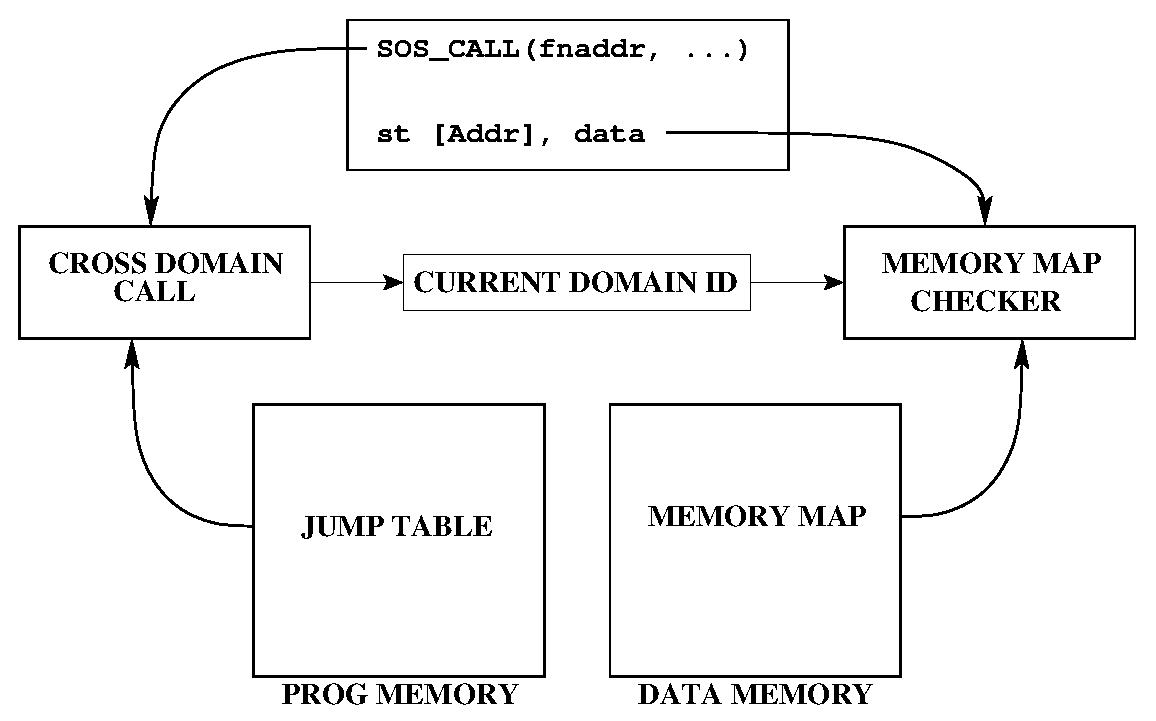
\includegraphics[height = 2.5in, keepaspectratio=true]{figures/syscomp.eps} 
%     \caption{Components of Harbor Memory Protection}
%     \label{fig:sys_comp}
%  \end{figure}

%-------------------------------------------------------
\subsection{Applications of Harbor Memory Protection}
%
\subsubsection{Memory Protection in SOS Operating System}
%
SOS~\cite{ram05sos} is an operating system for sensor nodes in which a
statically compiled kernel is installed on the node, and application
level functionality is implemented by a set of dynamically loadable
binary modules.
%
We use Harbor memory protection to isolate binary modules running
on SOS.
%
Run-time checks are introduced in a SOS module by a \emph{binary rewriter} and
verified independently by a \emph{verifier} running on every sensor
node.
%
To minimize the module code size, the run-time checks are not inlined.
%
Modules invoke the run-time checks by calling or jumping into the
appropriate routines located in the trusted domain (the SOS kernel).
%
%% Thus, it is not possible to circumvent checks as 
All potentially unsafe operations such as stores to memory are replaced
by calls to corresponding checks.
%
%Calls to the checks are introduced by a \emph{binary rewriter} and verified
%independently by a \emph{verifier} running on every sensor node.
%
Harbor's correctness depends only upon the correctness of the
verifier and the Harbor runtime, and not on the rewriter.
%
%The design of the verifier affects the system's performance
%(Section~\ref{sec:writeverify}).
%
%So far, we have only 
We have designed a simple verifier that requires constant state
information for a binary.
%
%Exploring the design space of verifiers and evaluating their impact on
%performance is a challenge that remains to be addressed.
%----------------------------------------------------------------------------
\subsubsection{Micro Memory Protection Unit}
%
We design a Micro Memory Protection Unit (UMPU) by partitioning the
Harbor Memory Protection system into hardware and software components.
%
UMPU was implemented on the AVR~\cite{avrdatasheet} microcontroller and
its performance was evaluated by executing complex software systems
such as SOS.
%
The careful hardware software co-design of UMPU results in significant
performance improvement over a software-only implementation with minimal
increase to the area and cost of AVR.
%
AVR enhanced with UMPU extensions is instruction set compatible with
regular AVR microcontrollers.
%
This design feature has practical value, as the existing
toolchains for the AVR architecture can be used with UMPU.
%
%
%An additional benefit of UMPU is that it eliminates the binary
%rewriting required by the software-only implementation that can be
%error-prone.
%


During experimentation, Harbor detected memory corruption in a data
collection application module that had been in use for several months.
%
A common programming mistake in SOS is to forget to check the error code
returned by a cross-domain function call.
%
In the Surge data collection module~\cite{woo03surge}, under certain
conditions, the invalid result of a failed function call to the Tree
routing module was being used to determine an offset into a buffer.
%
Subsequently, the data was being written to an incorrect memory
location, which would cause some of the nodes in the network to crash.
%
Harbor was successfully able to prevent the corruption and signal the
invalid access.
%


The cross-domain function call described above fails under the rare
condition when the Surge module is loaded on a node before the Tree
routing module.
%
Such conditions can be easily missed during software testing.
%
However, during deployments, the errors caused due to such failures
can have a severe impact on the network.
%
A system that can guarantee memory protection is indispensable for
building robust embedded software.
%

Harbor protection mechanism can be applied in general to a large class
of resource constrained embedded systems.
%
In this paper, we will focus primarily on the application of Harbor
protection to embedded sensor networks.
%
%----------------------------------------------------------------------------
%
%\subsection{Robust Embedded Software}
%
%============================================================
\subsection{Structure of Paper}
%
This paper is structured as follows.
%
Section~\ref{sec:related} gives an overview of related work,
examining previous work on software reliability in sensor networks,
software based fault isolation techniques and hardware based
approaches to memory protection in embedded and desktop systems.
%
%There is also a background on the SOS operating system. 
%and presents an overview of the Harbor memory
%protection primitives and their role in
%system that is designed to sandbox 
%sandboxing the dynamically loadable SOS modules.

Section~\ref{sec:memmap} explains the memory map data structure, which
contains fine grained ownership and layout information for every block
within the address space of the sensor node. 
%
Section~\ref{sec:cfmgr} discusses the Control Flow Manager, which
ensures the integrity of control flow within a protection domain
despite memory corruption localized to a domain.

Section~\ref{sec:writeverify} describes the design and implementation
of a binary rewriter tool that sandboxes SOS modules.
%
The sandboxed modules interact with the Harbor run-time components.
%
There is a detailed discussion on the design space of the verifiers
for a binary rewriter.

Section~\ref{sec:umpu} describes the components of UMPU.
%
There is an in-depth 
%detailed design 
description of all the functional units
within UMPU and their interaction with the software library.

We present detailed performance and resource consumption analysis of
Harbor and UMPU in Section~\ref{sec:eval}.
%
We conclude with a summary of our findings and directions for future
work in Section~\ref{sec:conclude}.

%=======================================================================
% RELATED WORK
%=======================================================================
\section{Related Work}
\label{sec:related}
%
Page-based virtual memory systems have become the dominant form of
memory management in the modern general-purpose computer systems.
%
While the process model of the virtual memory systems deliver protection for embedded applications, they also increase overhead in memory consumption and processor performance.
%
The memory consumption increases due to the need to store address translation tables.
%
The processor performance is impacted because the context switch has a high overhead; page tables have to be setup for the new context.
%
To improve performance of virtual memory, architectural features such as Translation Lookaside Buffers (TLBs) and virtual-mapped caches are used that further increase the area, cost and complexity of the chip.
%
For example, the addition of MMU and cache in an ARM7TDMI core~\cite{arm7tdmi} increases its area ten fold and its power consumption two fold. 
%
Therefore, current MMU designs will never be used in the low end price sensitive microcontrollers.

%
Memory protection units (MPU) provide hardware assisted protection in  embedded processors such as ARM
940T~\cite{arm940tds} and Infineon TC1775~\cite{inftc1775ds}.
%
MPU can statically partitions memory and set individual protection attributes for each partition.
%
The partitions are contiguous segments within the address space defined by a pair of base and bounds registers.
%
The protection model of MPU is not suited for the complex embedded
software (such as operating systems) running on low-end microcontrollers.
%
MPU defines only two protection domains viz. User-mode and Supervisor
mode.
%
This is sufficient for protecting the kernel from the applications but
not the applications from one another.
%
The static partitioning of address space into contiguous regions is
infeasible for the low-end microcontrollers with very limited memory
footprint.
%
Further, the number of partitions is also limited.
%
However, MPU has a lower memory footprint than UMPU because the
partitioning information can be stored in registers instead of
maintaining a memory map.
%
MPU introduces no performance overhead while UMPU incurs a single
clock cycle penalty for memory map accesses.
%


%
Mondrian Memory Protection (MMP)~\cite{witchel-asplos02-mondrian} inspects memory accesses at the instruction level from within the processor pipeline to provide word-level protection.
%
It uses fairly complex and expensive hardware extensions to reduce overhead of monitoring all accesses.
%
SafeMem~\cite{qin-hpca05-safemem} exploits existing ECC memory protection to guard memory regions and detect any illegal accesses through ECC violations.
%
However, these techniques significant resources to be performed on tiny embedded processors.

%
Hardware support for memory safe execution of embedded software was recently proposed in~\cite{divya06ccured}.
%
This technique uses CCured~\cite{ccured02necula}, a tool that generates type safe C programs through pointer inference techniques.
%
Extensions to the instruction set architecture speed up the run-time bounds checking operations performed by CCured.
%
Our techniques apply directly to machine instructions and are therefore agnostic to programming languages.
%
Also, our hardware extensions do not modify the processor instruction set architecture.
%
Hence, we can continue to use existing compilers.
%
Custom modifications to compilers can become the source of new bugs.
%

Many software based approaches for memory protection have been proposed.
%
Type-safe languages such as Virgil~\cite{titzer06virgil} can flag illegal accesses at compile or run-time.
%
They provide fine-grained memory protection of individual objects.
%
Type-safe languages do not interface with code written in non type-safe languages.
%
However, most of the software developed for embedded systems is written in unsafe languages such as C (or even assembly for low-level drivers). 
%
Popular programming language NesC~\cite{gay03nesc}, contains minimal extensions to C (such as the \texttt{atomic} keyword) to prevent race-conditions that can cause memory corruption.
%
ASVM~\cite{asvm05nsdi} can also be used for providing memory protection. 
%
Software-based fault isolation for embedded processors has been proposed in ~\cite{ram07harbor}.
%
All the software based approaches have a significantly higher overhead than custom hardware extensions.

%==========================================================================
% DESIGN COMPONENTS
%==========================================================================
\section{Memory Map}
\label{sec:memmap}
%
%==========================================================================
% PROTECTION DOMAINS
%==========================================================================
%
\subsection{Protection Domains}
%
Our \textit{fault model} for memory protection is the corruption of state belonging to a module caused due to illegal write operations made by some another module.
%
We create and enforce \emph{Protection Domains} within data memory address space of the embedded processor.
%
Protection domain refers to a fragmented but logically distinct portion of overall data memory address space (Figure ~\ref{fig:prot_domains}).
%
Every module stores its state in its own protection domain.
%
No assumptions are made about layout of state within a domain.
%
Modules are restricted from writing to memory outside their domain through run-time checks.
%
There is one single trusted domain in the system that is allowed to access all memory.
%

Protection models based on domains do not address all possible memory corruption faults in the system.
%
Modules can still corrupt their own state as it resides completely within a protection domain. 
%
This form of corruption, though undesirable, is less serious than corruption across domains.
%
If we have an operating system we can load the kernel image in its separate domain.
%
A stable kernel can always ensure a clean re-start of user modules when corruption is detected.
%
\begin{figure}[htbp]
   \centering
   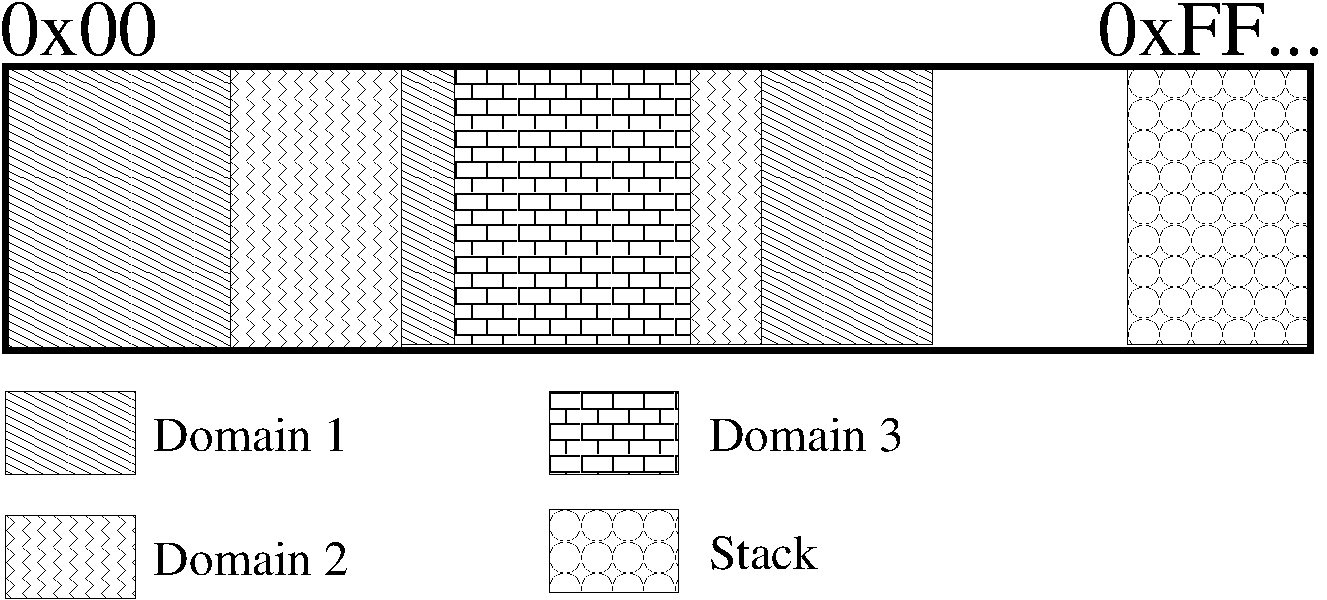
\includegraphics[height = 1in, keepaspectratio=true]{figures/domains.pdf} 
   \caption{Protection Domains}
   \label{fig:prot_domains}
\end{figure}
%
%========================================================================================================================================
% MEMORY MAP DATA STRUCTURE
%========================================================================================================================================
\subsection{Memory Map Data Structure}
%
%
Creating and enforcing protection domains is a challenging task on resource constrained embedded platforms.
%
Limited memory prohibits static contiguous partitioning of address space into multiple domains.
%
Instead we partition the address space of the microcontroller into blocks of equal sizes.
%
A \textit{Block} is a small contiguous region of memory.
%
Memory is allocated to domains as \textit{segments}, which are simply sets of contiguous blocks.
%
Allocation of segments to domains could be static (at compile time) or dynamic (through a memory heap).
%
A domain could be allocated multiple segments that are scattered randomly across entire address space.
%
\textit{The Memory Map contains access permissions for every block of address space.}
%
The Memory Map specifies two pieces of information.
% 
First, it contains ownership information (domain identity) for every block of memory.
%
Second, it encodes information about memory layout such as start of a logical segment of allocation to programs.
%
An example of actual encoded information and their meaning is specified in Table~\ref{tab:mmap_table}.
%
\begin{table}[htdp]
\centering
\small{
\begin{tabular}{|c|l|}
	\hline
	Code & Meaning\\
	\hline
	1111 & Free or Start of Trusted Segment\\
	1110 & Later portion of Trusted Segment\\
	xxx1 & Start of Domain (0 - 6) Segment \\
	xxx0 & Later portion of Domain (0 - 6) Segment\\
	\hline
\end{tabular}}
\caption{Encoded information in memory map table for multi-domain protection}
\label{tab:mmap_table}
\end{table}
%
%
%========================================================================================================================================
% MEMORY MAP CHECKER
%========================================================================================================================================
\subsection{Memory Map Checker}
%
A memory map checker is required to validate memory accesses made by software components.
%
It enforces the protection model that we described earlier; programs can write only into their domain.
%
The memory map checker is implemented as a functional unit (MMC) that intercepts the signals generated by the CPU for writing into the data memory (Figure~\ref{fig:mmcramcpu}).
%
If the write address is valid the MMC writes directly into the data memory.
%
\begin{figure}[htbp]
   \centering
   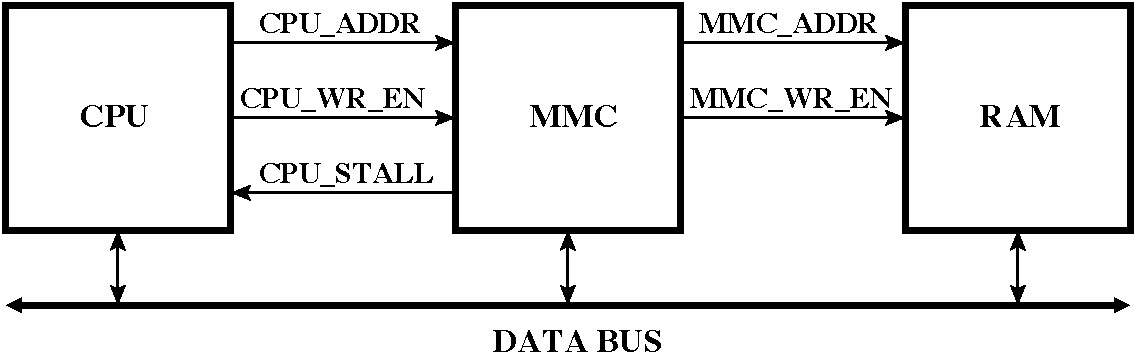
\includegraphics[height=0.5in, keepaspectratio=true]{figures/mmcramcpu.pdf} 
   \caption{Memory Map Controller (MMC)}
   \label{fig:mmcramcpu}
\end{figure}
%

The operations performed by MMC are three-fold.
%
First, it stalls the processor execution and takes control of the address bus to memory.
%
This occurs in the second cycle of the clock waveform shown in Figure~\ref{fig:mmcop}.
%
In the same clock cycle it performs an address translation operation to determine the address of the permissions in the memory map.
%
Address translation is shown in Figure~\ref{fig:memtrans}.
%
Memory map permissions are also read in this cycle as the MMC unit has control over the address bus.
%
Second, the MMC compares the ownership information to the identity of the current executing domain.
%
Finally, if the check is successful, then the MMC issues a write enable signal to the data memory.


The subset of address space protected by the memory map is defined by the register pair \texttt{mem\_prot\_bottom} and \texttt{mem\_prot\_top}.
%
The first step during translation is to determine the offset of the write address into the protected address space.
%
This is done by subtracting the lower bound of protected memory address space from the issued write address. 
%
Assuming a block size of 8 bytes, the nine significant bits of the address offset represent the block number.
%
Permissions are packed into a byte.
%
If the encoded information is stored in four bits (assuming multi-domain protection), then each byte would contain information of two contiguous memory blocks.
%
Therefore the last bit of the block number represents the byte offset of the permission.
%
The remaining bits index into the Memory Map Table.
%
The base pointer of the Memory Map Table is stored in a special register called \texttt{mem\_map\_base}.
%
The address of the permissions byte is computed by adding the memory map index to the memory map base pointer.
%
%
\begin{figure}[t]
  \centering
    \mbox{
      \subfigure[Timing]{\label{fig:mmcop}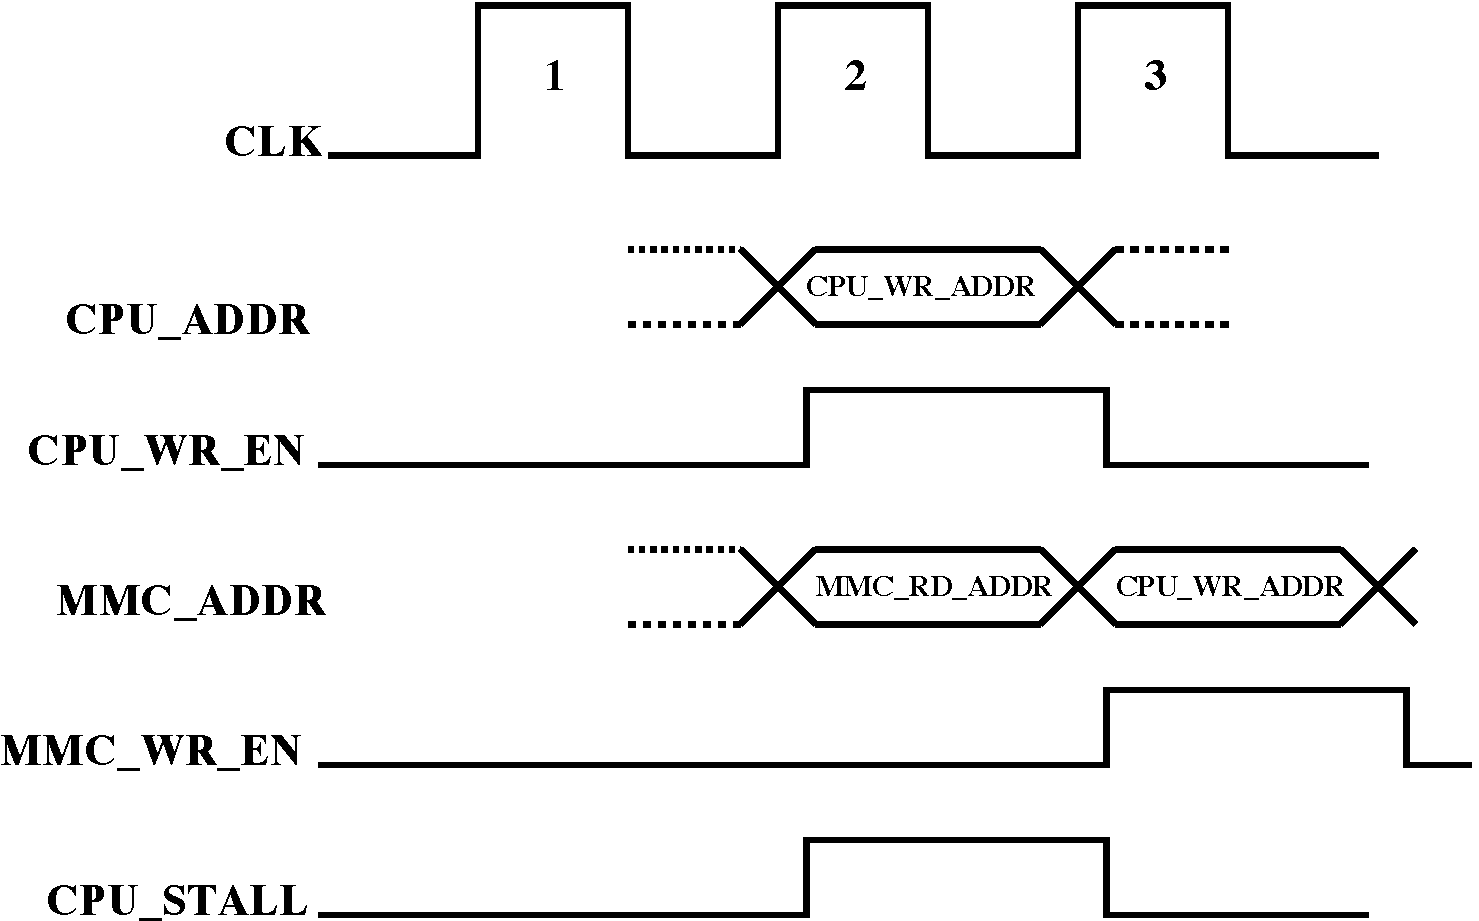
\includegraphics[height=1.2 in, keepaspectratio = true]{figures/mmcop.pdf}}\quad
      \subfigure[Addr Translate]{\label{fig:memtrans}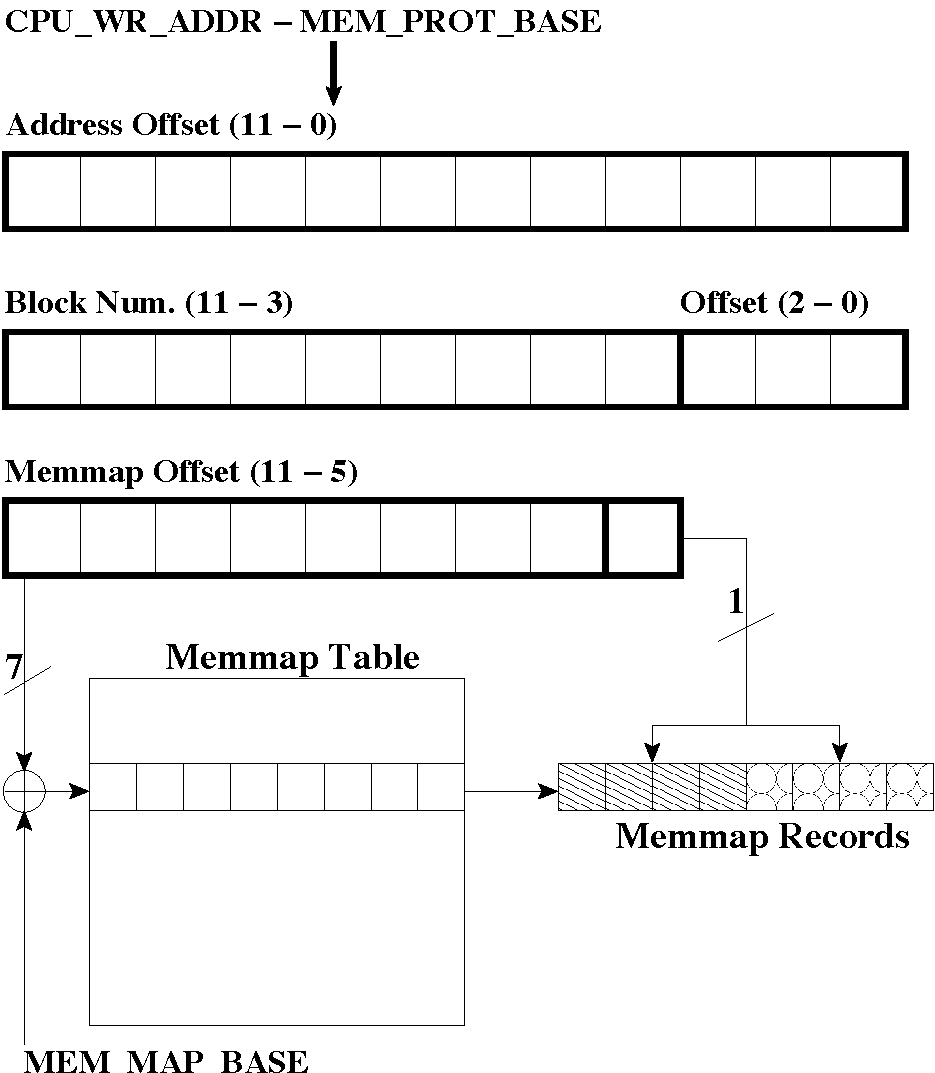
\includegraphics[height = 1.25in, keepaspectratio = true]{figures/memaddrtrans.pdf}}
    }
    \caption{MMC Operations}
    \label{fig:mmc}
\end{figure}

%
%
The Memory Map data structure is configurable through a set of programmable registers shown in Table~\ref{tab:mmap_config}.
%
The registers are accessible only by the run-time library loaded in the trusted domain.
%
The \texttt{mem\_map\_config} register is used to configure the block size and the number of protection domains available in the system.
%
\begin{table}[htdp]
\centering
\small{
\begin{tabular}{|l|l|}
	\hline
	Register & Function\\
	\hline
	\texttt{mem\_map\_base} & Memory map base pointer \\
	\texttt{mem\_prot\_bot} & Lower bound of protected address space\\
	\texttt{mem\_prot\_top} & Upper bound of protected address space\\
	\texttt{mem\_map\_config} & Configure block size and domains\\
	\hline
\end{tabular}}
\caption{Memory Map Configuration Registers}
\label{tab:mmap_config}
\end{table}
%
%========================================================================================================================================
% MEMORY MAP SOFTWARE LIBRARY
%========================================================================================================================================
\subsection{Memory Map Software Library}
\label{subsec:mmap_for_protection}
%
The software library manages all the memory available on the embedded processor.
%
First, it ensures that the memory map accurately reflects current ownership and layout.
%
In any real system, memory is constantly allocated, de-allocated or transferred from one module to another.
%
The Memory Map should be immediately updated when any of these events occur.
%
The library provides \texttt{malloc}, \texttt{free} and \texttt{change\_own} calls that automatically update the  Memory Map data structure. 
%
Second, it only permits the  block owner to free or change its ownership.
%
This condition is necessary as one module may (due to programming errors) free up memory that is being used by other module in the system.
%
Also it prevents a module from accidentally hijacking memory that is owned by other modules.
%
To enforce this condition, the software library reads the identity of the current active domain from the status register.
%
%We describe implementation details of tracking current active application in Section~\ref{sec:cfmgr}.
%
Third, the software library sets up the memory map to be located in a protected region of memory.
%
This prevents accidental corruption of the Memory Map data structure.
%
It is the responsibility of the software library to ensure that a memory map of sufficient size is allocated in the system.
%
Fourth, it initializes the MMC with the appropriate block size, number of protection domains and the range of protected address space.
%






\section{Control Flow Manager}
\label{sec:cfmgr}
%
Programming errors can cause a module to corrupt its own state, even with
protection domains.
%
%% The protection domains cannot
%% prevent such internal memory corruption.
%
Unfortunately, a user module's control flow might be affected by internal memory
corruption.
%
For example, function pointers (commonly used to implement callbacks)
are stored in RAM.
%
Return addresses to function call sites are stored in stack.
%
Corruption of these values might cause the processor to execute
arbitrary code, including the memory map API,
%
violating one of the requirements of using the memory map for
protection.
%% ; restricting memory map access to single trusted domain
%% (Refer Section~\ref{subsec:mmap_for_protection}).
%
The \emph{control flow manager} ensures that control can never flow out of
a domain except via calls to functions exported by the kernel or modules in
other domains, and via the corresponding returns.
%
Conversely, control flow can enter a domain only through an exported
function or through the return site of a call that was made to a
function exported by some other domain.
%
The control flow manager also tracks the identity of the currently
executing domain.
%
This information is required by the memory map checker to validate write
accesses.
%
Harbor's \emph{cross domain call} mechanism is used
to transfer control safely from a caller to a callee domain.
%
A corresponding \emph{cross domain return} mechanism restores control back to
a caller domain. 
%
Control flow integrity within a domain is preserved through a \emph{safe stack}
that stores return addresses.
%
%==============================================================================
% CROSS DOMAIN CALL
%=============================================================================
\subsection{Cross Domain Call}
\label{sec:crossdomcall}
%
%All function calls made across domains pass through a \textit{cross domain call stub}.
%
%Four operations are performed by the cross domain call stub.
%
%
A cross domain call performs four operations.
%
First, it verifies the call's target address, which
%
should match the address of a function officially \emph{exported} by some
module or the kernel.
%
Second, it saves the caller's domain identity and return address.
%
Third, it sets up a \emph{stack bound}, which prevents the callee from
modifying portions of the stack belonging to the caller.
%
Finally, it jumps to the callee.
%
%% Stack bound is required for run-time stack protection (Section~\ref{subsec:stackguard}).
%
The cross domain call mechanism tries to optimize the performance of these operations.
%

\begin{figure}[htbp]
   \centering
   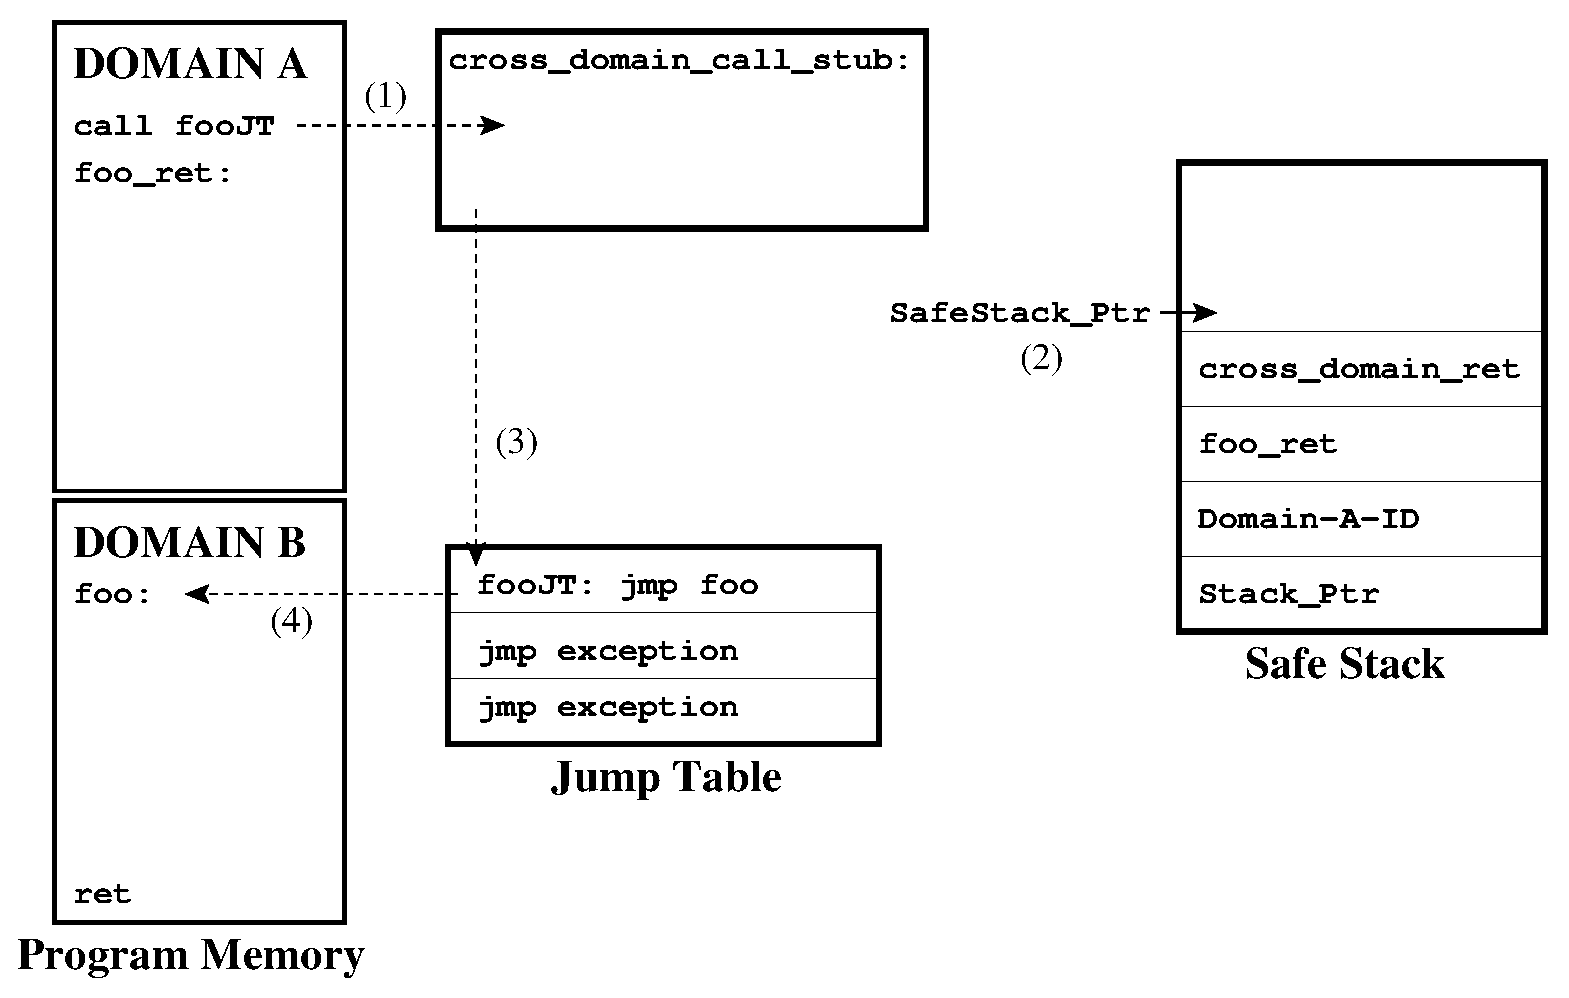
\includegraphics[height=2.0in, keepaspectratio=true]{figures/cross_domain_call_step.eps} 
   \caption[Cross domain call operation]{Cross Domain Call: (1) Control flow enters cross domain
     call stub (2) Stub stores domain ID, stack bound and return
     addresses on the safe stack (3) Stub jumps into an address in
     jump table (4) Jump table redirects to call implementation in new
   domain}
   \label{fig:cross_domain_call}
\end{figure}


%
Call address verification is accomplished with the help of a \emph{jump
table}, an extra level of indirection in cross-domain function calls.
%
%% This simplifies the verification of call target addresses
%% and eases the tracking of the system's currently active domain.
%
Modules in a domain are linked with modules in other domains at
load-time as described in Section~\ref{sec:soslinking}.
%
A linker running on the sensor node parses the module's exported functions
and writes them to the jump table.
%
The jump table, which is stored in flash memory, is similar in design
to an interrupt vector table.
%
Each jump table entry is an instruction to jump to an exported
function;
%
the function's address is encoded within the instruction stream.
%
Each domain has its own jump table, containing all the functions exported
by modules in that domain (or, for the kernel domain, all functions
exported by the kernel).
%
Since modules cannot directly write to flash memory, they cannot
corrupt the jump table.
%
Modules that subscribe to functions exported by a particular module
are redirected through the corresponding domain's jump table.
%
This is illustrated in Figure~\ref{fig:cross_domain_call}.
%
The jump table mechanism is independent of the process used for
dynamic linking (exporting and subscribing to functions), which might use
several other techniques~\cite{dunkels06linking}.
%

Each domain is currently allocated one page of internal flash memory for
storing its jump table.
%
%%%% XXX EDDIE STOPS HERE
%
In the AVR architecture, this imposes a limit of 64 exported functions per
domain.
%
The SOS kernel domain exports the system call API that consists of 32
functions.
%
SOS module currently export up to a maximum of 12 functions, allowing
at least 5 modules to share a domain.
%
Empty entries in the jump table are filled with a jump instruction to an
exception routine.
%
All domains' jump table pages are stored contiguously in flash memory,
reducing the overhead of verifying a call's target address and domain.



All function calls made across modules need to pass through a
\textit{cross domain call stub}.
%
This stub, a part of the Harbor runtime, is located
in a trusted region of program memory.
%
In SOS, cross module calls use a macro \texttt{SOS\_CALL};
%
we modified its implementation to force
a call into the cross domain call stub.
%
This is implemented as an assembly routine
within the SOS kernel, with pseudocode
%
shown in
Figure~\ref{fig:cross_domain_call_stub}.
%
\begin{figure} [h]
  \centering
\begin{tiny}
\begin{verbatim}
cross_domain_call_stub(addr_t addr) {
   // Store current return addr in safe stack
   push_ss ret_addr

   // Check if target address is valid
   if (addr > JMP_TBL_BASE) { 
      // Store current state in safe stack
      push_ss curr_domain_id;       
      push_ss curr_stack_bound;
 
      // Compute new domain ID
      curr_domain_id = MSB((addr - JMP_TBL_BASE) << 1);
      if (curr_domain_id > MAX_DOMAIN_ID)
         control_flow_exception();
                 
      // Compute new stack bound (For run-time stack protection)
      curr_statck_bound = STACK_PTR;
     
      // Push the return address of cross domain return
      push_ss cross_domain_return
     
      // Call into jump table
      call addr;
     
cross_domain_return:
      // Restore previous state
      pop_ss curr_stack_bound
      pop_ss curr_domain_id
     
      // Return to caller domain
      ret    
  } else
    control_flow_exception(); 
}
\end{verbatim}
\end{tiny}
\vskip-\baselineskip
  \caption{Pseudocode of Cross Domain Call Stub}
  \label{fig:cross_domain_call_stub}
\end{figure}
%

The stub first stores the return address in the safe stack (Section~\ref{subsec:safe_stack}).
%
%% The design of safe stack is described later in
%% Section~\ref{subsec:safe_stack}.
%
All valid cross-module calls must have target addresses that reside in the
jump table, since
%
modules subscribe to jump table locations
corresponding to the functions exported by other modules.
%
A call into the jump table is checked by a simple compare operation to
the base address of jump table.
%
%% Check against the upper bound of jump table is deferred.
%
The stub then stores the current domain identifier and the stack bound
in the safe stack.
%
A store into the stack is required because cross domain calls can be
chained: domain A calls domain B, which in turn calls domain C.
%
Next, the identity of the callee domain is computed by determining
the jump table page in which the target address falls.
%
%% Jump tables of all domains are organized linearly, starting from the
%% domain 0 jump table located at the base address.
%% %
%% The identifier of target domain can be easily determined by first
%% computing the address offset from the base address of jump table and
%% dividing it by the size of jump table.
%
If the target domain identifier exceeds the maximum number of domains
in the system, then the target address is greater
than the upper bound of jump table; an exception is generated.
%
The callee domain may equal the current domain when a module transfers
control to another module in the same domain.
%
The cross domain return address is pushed to the safe stack, ensuring that
%
control flow will return to the stub.
%
Finally, a call is made into the jump table, which redirects it to the
actual entry point in the target domain.
%
During cross domain return, the previous domain identifier and stack
bound are restored and the control is transferred back to caller
domain.
%

As all domains share a common run-time stack, the cross
domain call stub does not need to copy call arguments.
%
Further, no modifications are made to any data frames set up in the run-time
stack during function calls.
%
Therefore, a single cross domain call and return stub suffices for
all cross domain calls, unlike the per-function stub required by the
original SFI~\cite{wahbe93sfi}.
%
The implementation of the cross domain call stub only uses the
caller-saved registers described by the \texttt{avr-gcc} ABI.
%

Harbor currently disallows all computed branches except for cross
module calls.  This ensures that applications cannot avoid memory and/or
control flow checks, but also prevents certain implementations of control
flow structures like \texttt{switch}.


%==============================================================================
% STACK PROTECTION
%==============================================================================
\subsection{Run-Time Stack Protection}
\label{subsec:stackguard}
%
%% Micro-controllers have a single address space and therefore the
%% run-time stack is shared by entire system.
%% %
%% In most architectures, stack is initialized at the end of address
%% space and grows down towards the start of address space.
%% %
%% Run-time stack is used for many purposes.
%% %
%% First, it is used to record return addresses of function calls.
%% %
%% Second, it is used to set up data frames for storing local variables
%% or function arguments that cannot be accommodated in registers.
%% %
%% Third, it is also used to store arguments for variadic functions.
%% %

Harbor shares a common run-time stack across all domains.
%
The design alternative, allocating a private stack per domain,
%
would require too much memory, since stack memory must be allocated
conservatively (the stack can grow significantly during execution).
%
%% Therefore, this design is not feasible on micro-controllers.
%
%% However, stack corruption is a serious problem when it is shared
%% across domains.
%
Harbor implements a \emph{stack bound} to prevent one domain from
corrupting another domain's local variables and other stack
information.
%
The cross domain call stub sets up a stack bound before transferring
control, and the cross domain return stub restores the previous stack
bound.
%
The stack bound is set to the beginning of the callee frame as shown
in the Figure~\ref{fig:stackbound}.
%
As shown in Figure~\ref{fig:checker}, the stack access checker is invoked
for writes to the run-time stack, a statically allocated region of memory
at the high end of the address space.
%
Harbor disallows writes to memory addresses greater than the current stack
bound (assuming a stack that grows down).
%
%% The stack access checker compares the write address to the current stack
%% bound and signals an exception if the address exceeds the stack bound.
%
%% Therefore, a module cannot corrupt the stack belonging to another domain.
%
%% As mentioned in Section~\ref{subsec:cdc}, the current stack bound is
%% updated by the cross domain call and return stubs.
\begin{figure}[htbp]
   \centering
   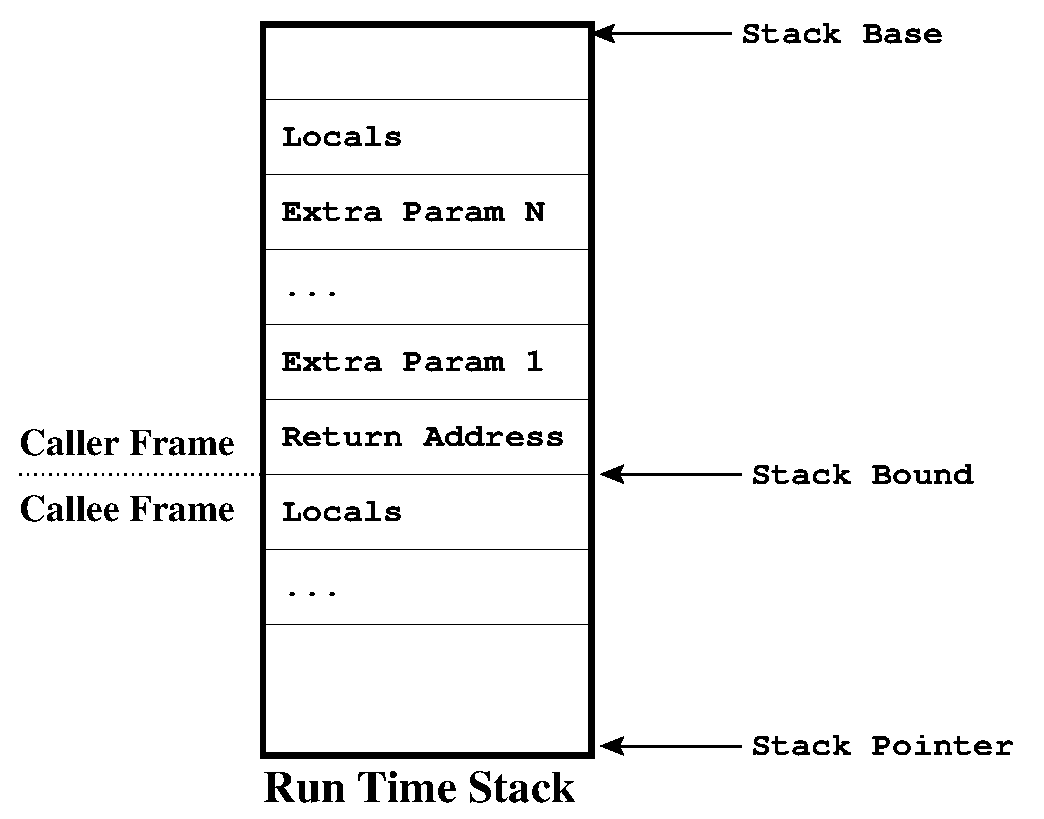
\includegraphics[height=2.0in, keepaspectratio=true]{figures/stack_bounds.eps} 
   \caption[Run-time stack protection using stack bounds]{Run-time stack protection using stack bounds. All writes
     above the current stack bound are disallowed.}
   \label{fig:stackbound}
\end{figure}


The stack bound does prevent cross domain data sharing through the stack,
but we have never encountered an instance of such sharing
in the SOS system.
%


%=============================================================================
% SAFE STACK
%==============================================================================
\subsection{Safe Stack}
\label{subsec:safe_stack}
%
Correct fault isolation requires that Harbor limit control flow
\emph{within} modules, as well as across modules.
%
A module must not be able to jump into its code arbitrarily, since this
might allow it to avoid a run-time check.
%
The Harbor runtime therefore uses an additional \emph{safe stack}
to preserve the integrity of control flow within and across modules.
%
The safe stack resides in the
trusted domain, preventing any corruption by application wild writes.
%
%% This prevents any corruption to the safe stack caused due to wild
%% writes.
%
%% Only the code executing in the trusted domain can access the safe
%% stack.
%
Harbor stores function calls' return addresses on the safe stack,
protecting them from wild writes by applications in any domain
(Figure~\ref{fig:safestack}).
%
The cross domain call stub also uses the safe stack to store the current
domain ID and run-time stack bound.
%
The safe stack pointer is maintained as a global variable, and manipulated
by sequences of push and pop operations.
%%  is read
%% (and written) before (and after) a sequence of push/pop operations. 
%
%% A module can call any local function within its domain.
%
%% The return addresses of function calls are stored in the run-stack and are
%% protected from corruption from modules in other domains.
%
%% However, a programming error can cause a module to corrupt its own
%% run-time stack.
%
%% This cannot be prevented by protection domains.
%
%% Executing the return instruction on the corrupted run-time stack can cause the
%% control flow to become unpredictable.
%
%% Therefore, Harbor stores all return addresses within the safe stack.
%
A function entry stub, \texttt{func\_entry\_stub}, copies the return
address from the run-time stack onto the safe stack.
%
Similarly, \texttt{func\_exit\_stub} pops the return address from
the safe stack and restores the run-time stack.
%
The entry and exit points of every local function within a domain are
rewritten to invoke these stub routines.
% in the trusted domain that pushes
%(and pops) return addresses into the Safe Stack.
%
%
%Safe Stack is used to overwrite return address values in run-time
%stack.
%
We do not modify the run-time stack in any manner as this would corrupt data
frames setup by functions for storing local data and function
arguments.
%
\begin{figure}[htbp]
   \centering
   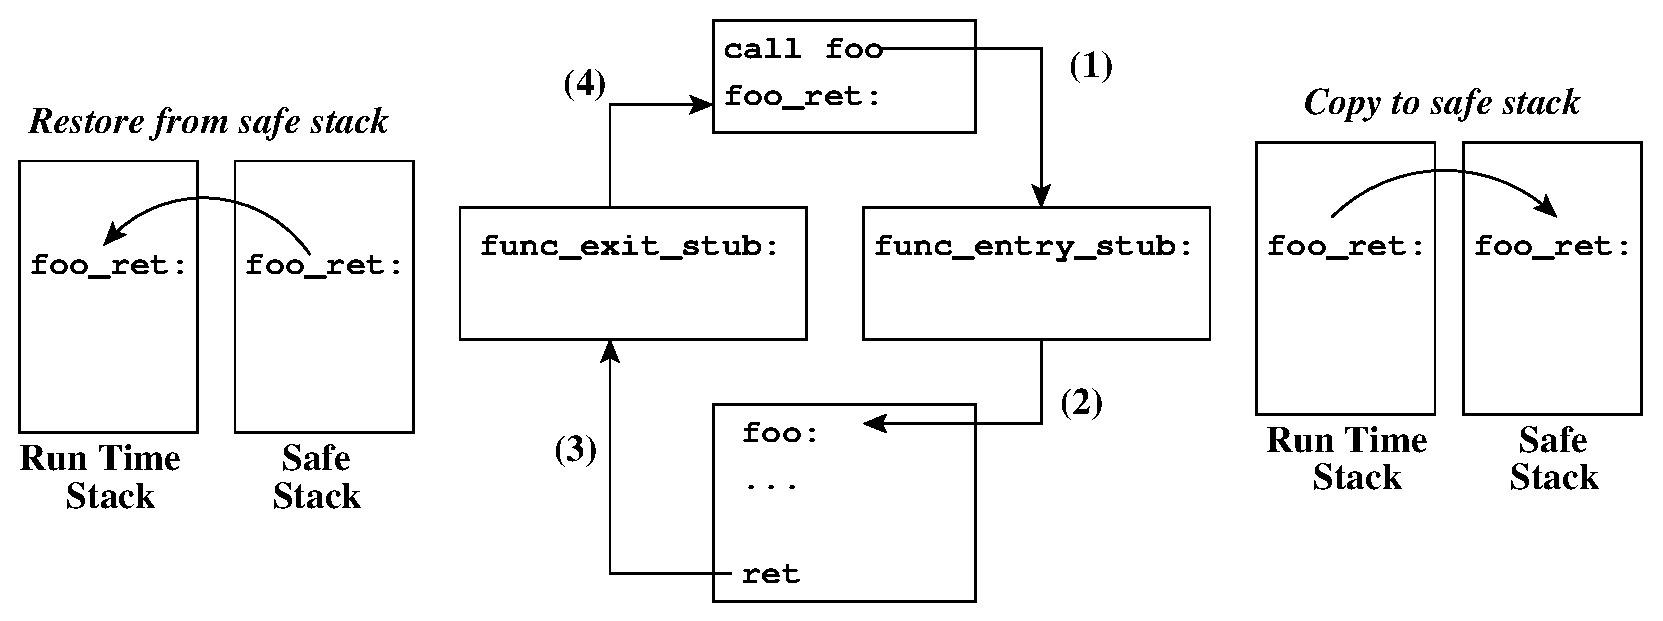
\includegraphics[width=5.3in, keepaspectratio=true]{figures/safe_stack.eps} 
   \caption[Using safe stack for storing return address]{Using safe
     stack for storing return address (1) All calls are redirected
     into the \texttt{func\_entry\_stub} (2) The stub copies return
     address from run-time stack to safe stack (3) All returns are
     redirected into the \texttt{func\_exit\_stub} (4) The stub
     restores copied return address from safe stack to run-time stack}
   \label{fig:safestack}
\end{figure}

The safe stack can be placed anywhere in data memory as long as it is
protected from accidental writes and overflow.
%
We usually place the safe stack at the end of all global data in the
system and make it grow upwards.
%
The run-time stack and safe stack thus approach one another.
%
%Therefore, all return addresses are checked.
%
%Domains occupy contiguous portions in program memory. 
%
%When the domain is loaded into a system, the Control flow manager records its start and end addresses.
%
%Return addresses are checked to ensure that they lie within bounds of the current domain; else an exception is raised.
%
%Similarly, all computed call addresses are also subject to an identical bounds check.
%
%Calls to static addresses are verified at load time.
%
%All checks are introduced through a binary rewriter.

%==============================================================================================
% SECTION BINARY RE-WRITER AND VERIFIER
%==============================================================================================
\section{Harbor Memory Protection for SOS}
\label{sec:writeverify}
In this section we describe the design of a system that provides
protection in the SOS operating system by sandboxing dynamically
loadable modules.
% 
\subsection{System Components}
% 
The components of a sandbox system are shown in Figure~\ref{fig:sys_overview}.
% 
%% We first describe overall system operation.
% 
The sandbox system's input consists of SOS module binaries generated by a
cross-compiler toolchain.
% 
The \emph{binary rewriter} is a desktop application that statically
analyzes these binaries for potentially unsafe operations and invokes
run-time checks to sandbox them.
% 
The sandboxed binary is then distributed to a network of sensor nodes.
% 
%A \emph{verifier} running on each node verifies that incoming binaries
%are correctly sandboxed.
% 
A \emph{verifier} running on each node inspects the sandboxed binary
to ensure that sufficient checks have been introduced to prevent any
possible protection violation.
%
Verified binaries admitted for execution interact closely with
Harbor's run-time components, the \emph{memory map manager} and
\emph{control flow manager}.
%
\begin{figure}[htbp]
  \centering
  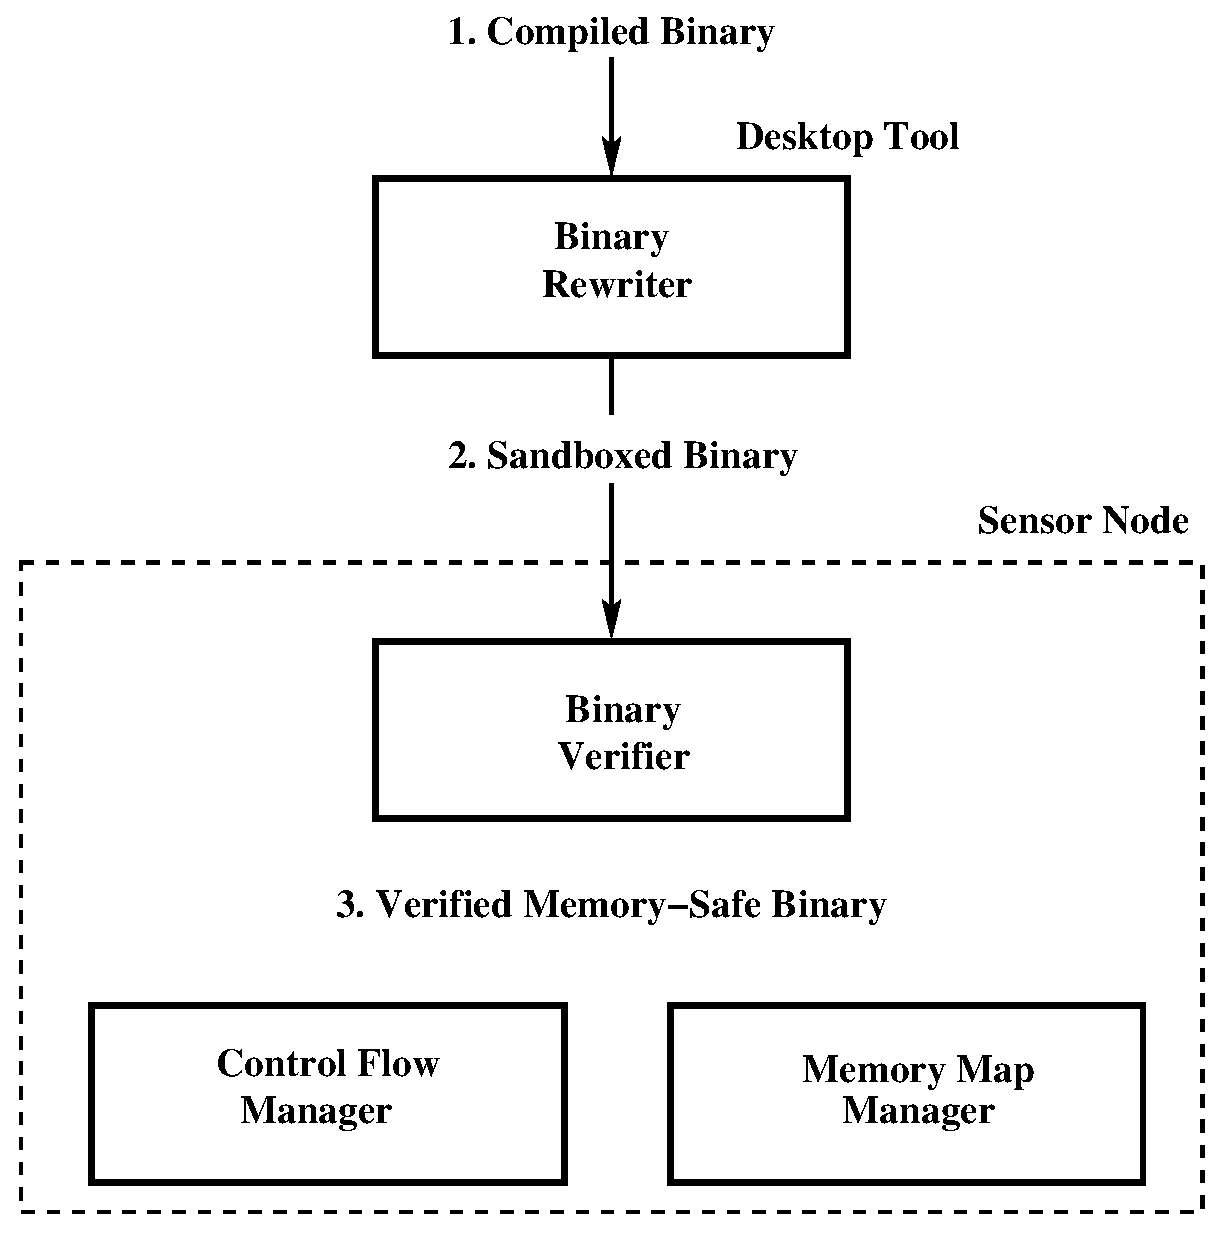
\includegraphics[height = 2.0in, keepaspectratio=true]{figures/sysoverview.eps} 
  \caption{Sandbox System Overview}
  \label{fig:sys_overview}
\end{figure}

%
As described in Section~\ref{sec:mmapchecker}, memory protection is
established through run-time checks. 
%
%In this section, we discuss a system that introduces these checks by
%rewriting the binaries produced by a cross-compiler toolchain.
%
The routines that implement the checks are located in the trusted
domain.
%
%The rewriter introduces calls and jumps that invoke the runtime
%checks from the sandboxed binary.
%
%
The verifier and rewriter are completely independent, and
%
the node that executes a sandboxed binary needs to trust only the
verifier.
%
The verifier could be a desktop application that, for example,
cryptographically signed binaries, or a trusted component running on the
sensor node.
%
%% If the verifier is a desktop application, the verified binary needs to
%% be cryptographically signed before being injected into the network.
%
%% The node needs to verify the cryptographic signature of a binary
%% before it is admitted for execution.
%
Our verifier is a trusted component running on every sensor
node that verifies sandboxed binaries locally prior to admitting them
for execution.
%
Sandboxed binaries can be seen as an example of proof-carrying code
(PCC)~\cite{necula96pcc}, even though they do not include any logical
proofs.
%
An attractive feature of this architecture is that sensor nodes do not
need to trust any external component.
%
%We discuss the tradeoffs involved in the design of the verifier in
%Section~\ref{sec:verifydesignspace}.
%
%==============================================================================
% INLINE CHECKS
%==============================================================================
\subsection{Sandboxed Operations}
%
Five types of operations are protected by the sandboxer.
%
\begin{enumerate}
%
\item{All forms of store instructions are sandboxed by a call to the
memory map checker.}
%
\item{All function call entry points are instrumented with calls to
the function entry stub, which uses the safe stack.}
%
\item{All return instructions are redirected to the function exit stub.}
%
\item{All computed calls are redirected to a stub that checks if
the destination is in the jump table.} 
%
\item{The beginning of each basic block is marked by a special
\texttt{NOP} symbol.}
%
\end{enumerate}

An example of the sequence of instructions introduced by the rewriter for
the AVR architecture is shown in Figure~\ref{fig:inlinechecks}.
%
The sequence is re-entrant; it can be preempted by interrupts.
%
%Push and pop instructions used in sandboxing store instructions can be removed by using dedicated registers.
%
%However, the AVR-GCC register allocator does not support using dedicated registers.
%
The rewriter performs a basic block analysis of the binary and preserves
the program's original control flow by updating static jump, call, and
branch targets.

\begin{figure}[htbp]
   \centering
   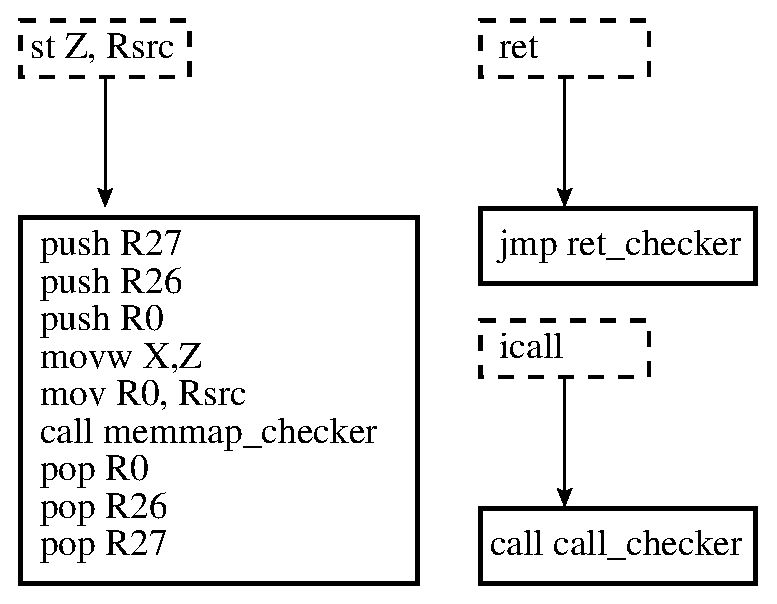
\includegraphics[height=1.75in, keepaspectratio=true]{figures/rewriter.eps} 
   \caption{Inline Checks}
   \label{fig:inlinechecks}
\end{figure}
%

The rewriter reads ELF object files.
%
It uses symbol table information to
distinguish binary data representing code and constants.
%
Upon sandboxing, the rewriter outputs a new ELF object file.
%
The symbol table and the relocation records in the output ELF file are
suitably modified to reflect their updated positions within the
sandboxed code.
%
Since linkers such as \texttt{avr-ld} link object files in ELF format,
%
the binary rewriter can be used to sandbox only portions
of the complete binary.
%
For example, only the device drivers in the final image of an
operating system might be sandboxed before installion.
%

%
%
%==============================================================================
% VERIFIER
%==============================================================================
\subsection{Verifier}
%
The verifier is a very simple program that maintains constant state
independent of the size of the binary.
%
In Harbor, all potentially unsafe operations, such as store to
memory, returns, and computed calls, are performed within the
run-time checkers.
%
Therefore, the verifier performs a single pass over the entire
instruction sequence and raises an exception if it encounters
any of the potentially unsafe operations. 
%such as stores, returns and computed call/jump instructions.
%
It checks all static jump, call, and branch targets to ensure that
they are within domain boundaries.
%
It also ensures that these targets point to valid instructions.
%
This check is necessary because AVR ISA has multi-word instructions.
%
If control flow jumped into the middle of a multi-word instruction,
run-time checks might be circumvented.
%
Therefore, the rewriter marks the beginning of basic blocks with a special
\texttt{NOP} symbol.
%
The verifier checks that all static jump, call, and branch targets
point to a \texttt{NOP}, and checks that the \texttt{NOP} symbol never
appears in the middle of a multi-word instruction.
%
%% The basic blocks are marked by a special \texttt{NOP} symbol; which is
%% checked to ensure to appear elsewhere in the 
%% %
%% Therefore, control flow can jump into the middle of a multi-word
%% instruction and circumvent the run-time checks.
% 
%Our current implementation of the verifier does not detect this.}
%
Function entry points (determined from call instruction targets) are
checked to ensure that they store the return addresses on the safe stack.
%
Finally, the verifier does not permit store instructions that write to
program memory.
%
The verifier calls an exception handler if any of these properties are violated.
%
%Its total line count is only 211 lines.
%
%----------------------------------------------------------------
% \section{Verifier Design Tradeoffs}
% \label{sec:verifydesignspace}
% The Harbor design also allows trading off execution overhead, and code size
% increase, against the complexity of the verifier.
% %
% Performance and code size increase are directly proportional to the
% number of operations that are sandboxed.
% %
% The current implementation sandboxes \textit{all} unsafe operations.
% %
% This severely penalizes performance and code size but reduces the
% complexity of the verifier, which requires only a single pass over the
% entire binary and maintains no additional state.
% %
% Static analysis on the binary can reduce the number of operations
% sandboxed by adding single checks that safely protect a series of
% potentially unsafe operations.
% %
% However, the safety of such a check is harder to verify using a simple
% verifier.
% %A single check can be used to protect a series of potentially unsafe operations.
% %
% %A complex verifier can permit direct execution of potentially unsafe operations (such as stores) that have been protected by earlier checks.
% %
% An interesting area of future work is to explore this design space to
% develop a rewriter--verifier combination that consumes limited
% resources but improve performance, and reduces code size, of sandboxed
% binaries.

%%%%%%%%%%%%%%%%%%%%%%%%%%%%%%%%%%%%%%%%%
% UMPU
%%%%%%%%%%%%%%%%%%%%%%%%%%%%%%%%%%%%%%%%%
\section{Micro Memory Protection Unit}
\label{sec:umpu}
%
A completely software-based approach to memory protection incurs a
large performance penalty despite the performance optimizations
(Section~\ref{sec:bitmasklut}).
%
A detailed discussion of the overheads can be found in
Section~\ref{sec:eval}.
%
The additional CPU cycles introduced due to the run-time checks in
Harbor may not be tolerable in certain performance sensitive
applications such as Vango~\cite{ben06vango}.
%
In this section, we extend the ideas of Harbor memory protection to
design a memory protection unit for tiny embedded processors
%
%Tiny embedded processors refers to the severely resource constrained
%8-bit and 16-bit microcontrollers 
commonly found in mote class sensor nodes%.
%
%Examples of such microcontrollers are 
such as Atmel's ATMEGA128L~\cite{avrdatasheet} or TI's
MSP430~\cite{mspdatasheet}.


We present Micro Memory Protection Unit (UMPU) that is designed for
resource constrained tiny embedded processors.
%
Our approach is motivated by the fault isolation principles of Harbor
and is fundamentally different from memory protection units found in
some of the higher-end embedded processors (Section~\ref{sec:mpu}).
%
We do not partition the address space of the microcontroller.
%
Available memory on microcontrollers is severely limited.
%
For example, ATMEGA128 AVR has only 4 KB of on-chip RAM.
%
In most systems~\cite{hill02micro}, this is the total available memory.
%
Static partitioning would further limit the memory that is available
to individual software components.
%
Instead we rely on Harbor's Memory Map data structure to efficiently
record ownership and layout information of the entire address space.
%

The key difference between UMPU and any software-based fault isolation (SFI)
system is that UMPU does not rewrite binary to introduce run-time
checks.
%
UMPU instead enhances the implementation of \texttt{store, call} and
\texttt{return} instructions in the microcontroller to perform
run-time checks in hardware.
%
This minimizes the performance overhead of performing run-time checks
in software and also eliminates the binary rewrite step of SFI which
can be quite error prone.

\begin{figure}[htbp]
   \centering
   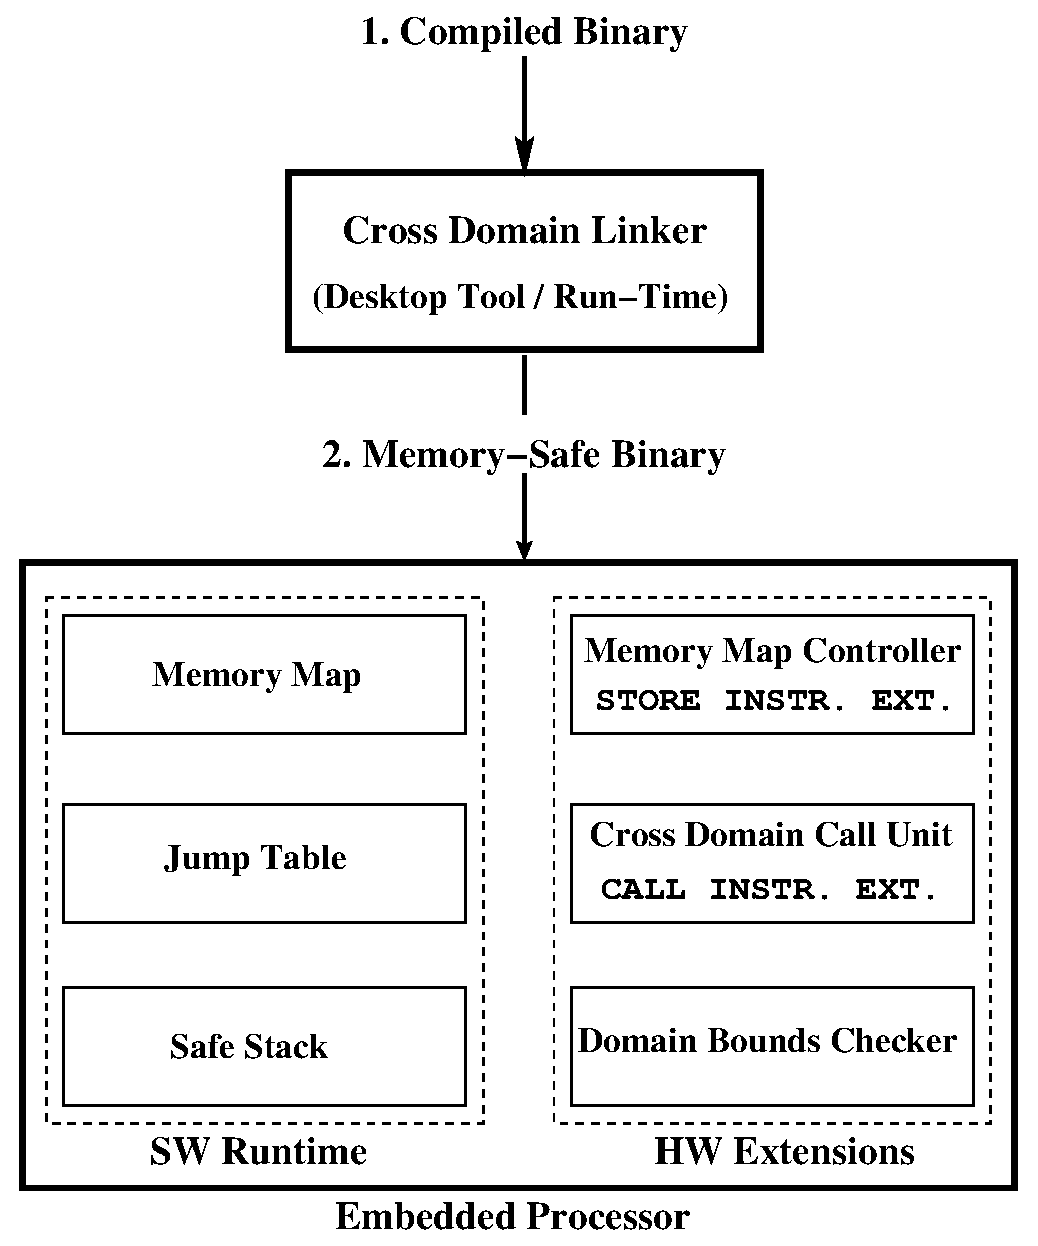
\includegraphics[height = 2.0in,
   keepaspectratio=true]{figures/umpuoverview.eps} 
   \caption{UMPU Overview}
   \label{fig:umpuoverview}
\end{figure}
%
UMPU can be viewed as a hardware software co-design approach to memory
protection (Figure~\ref{fig:umpuoverview}).
%
Low cost architecture extensions and a software run-time library work
together to isolate different software components running on an
embedded processor.
%
UMPU can be implemented entirely in software (as shown in already)
albeit a performance overhead.
%
Simple enhancements to the microcontroller core enable us to perform
critical operations in hardware thereby improving performance
significantly.
%
%-----------------------------------------------------------
\subsection{UMPU Overview}
%
An overview of our system highlighting all its components is shown in
Figure~\ref{fig:umpuoverview}.
%
The final firmware image is composed of multiple software modules that
need to be protected from one another.
%
%The software components are installed in separate protection domains.
%
A cross domain linking mechanism described in
(Section~\ref{sec:cross_domain_linking}) installs the software modules
in separate protection domains.
%
The cross domain linker generates a software jump table that assists
the domain tracker within the processor in determining the identity of 
the currently active domain.
%
The Control flow controller (Section~\ref{sec:cfctrl}) ensures control flow integrity through a cross domain call unit and a domain bounds checker.
%
A safe stack located in protected memory stores UMPU state information during cross domain calls.
%
Memory map (described in Section~\ref{sec:memmap}) tracks layout and ownership information for the protected address space.
%
The firmware image running on the processor, checked by the  memory map controller (Section~\ref{sec:mmc}) is guaranteed to be memory safe.
%
%The safe stack stores the return addresses in protected memory and 
%ensures control flow integrity within a module.
%

Upon reset, the processor boots into the trusted domain.
%
The code executing in the trusted domain is not subject to any checks.
%
The software library in the trusted domain configures UMPU by
initializing the configuration registers.
%
It also initializes the memory map.
%
The UMPU configuration registers are made read only when the control
flow leaves the trusted domain thereby avoiding any chance of
corruption.
%
The protection is enabled by setting the \texttt{UMPU\_EN} bit in the
\texttt{umpu\_config} register.
%
%
%-----------------------------------------------------------
\subsection{Memory Map Controller}
\label{sec:mmc}
%
Memory map controller (MMC) is a functional unit that interacts with
the memory map to validate memory accesses made by software
components.
%
It enforces the protection model that we described earlier; programs
can write only into their domain.
%
MMC intercepts the signals generated by the CPU for writing into the
data memory (Figure~\ref{fig:mmcramcpu}).
%
If the write address is valid, then the MMC writes directly into the
data memory.
%
\begin{figure}[htbp]
   \centering
   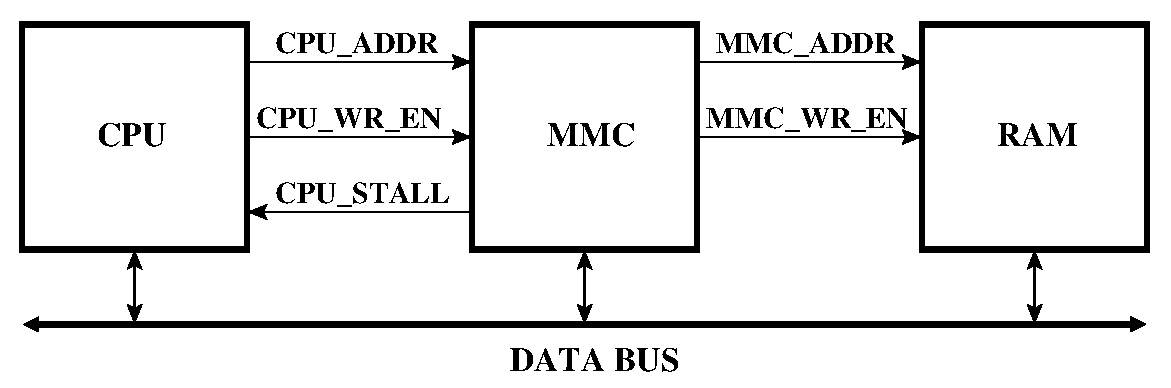
\includegraphics[height=1in,
   keepaspectratio=true]{figures/mmcramcpu.eps} 
   \caption{Memory Map Controller (MMC)}
   \label{fig:mmcramcpu}
\end{figure}
%
\begin{figure}[htpb]
 \centering
  \mbox{
    \subfigure[Regular Store]{\label{fig:mmcopst}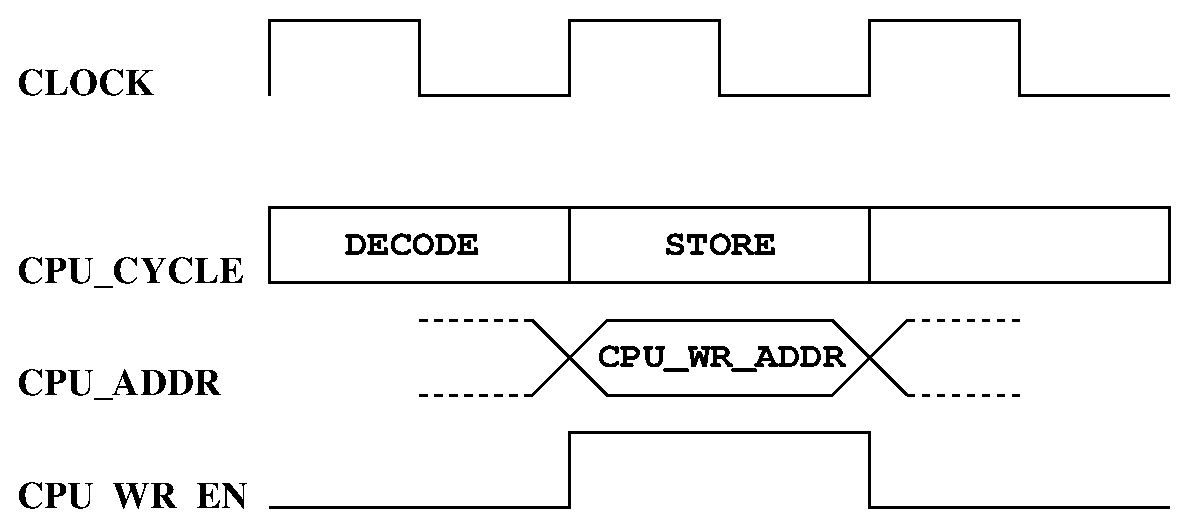
\includegraphics[width=2.5in,
      keepaspectratio = true]{figures/mmcop_st.eps}}
    \hspace{0.2in}
    \subfigure[Safe Store]{\label{fig:mmcopsafest}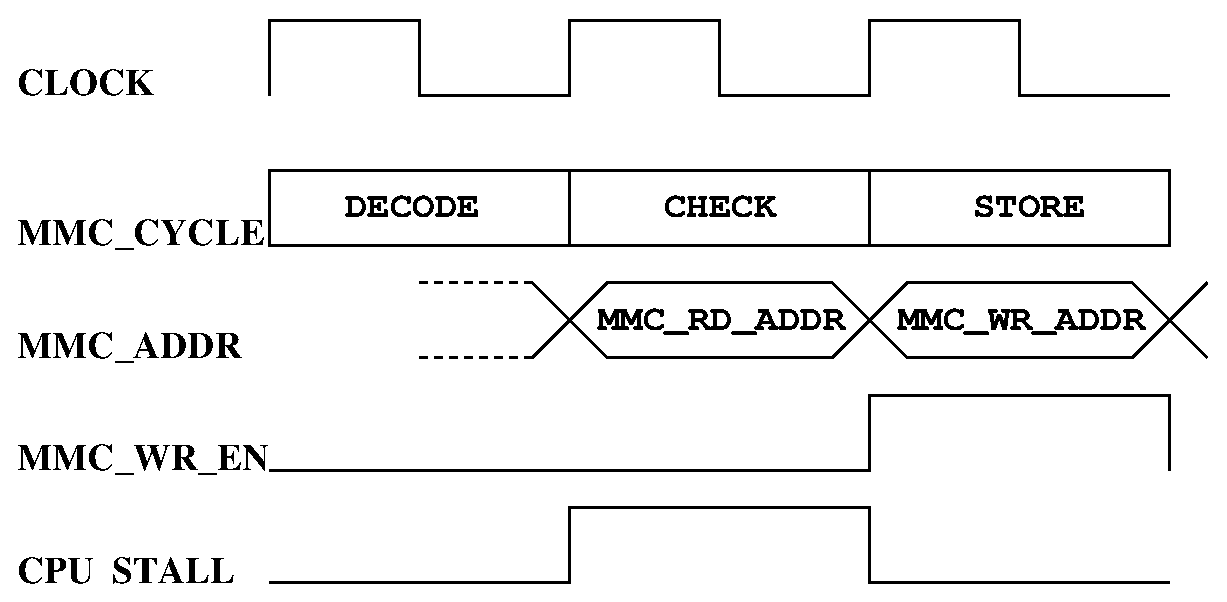
\includegraphics[width=2.5in,
      keepaspectratio = true]{figures/mmcop_safe_st.eps}}
  }
  \caption{MMC Timing Diagram}
\end{figure}   
% %
% \begin{figure}[htbp]
%    \centering
%    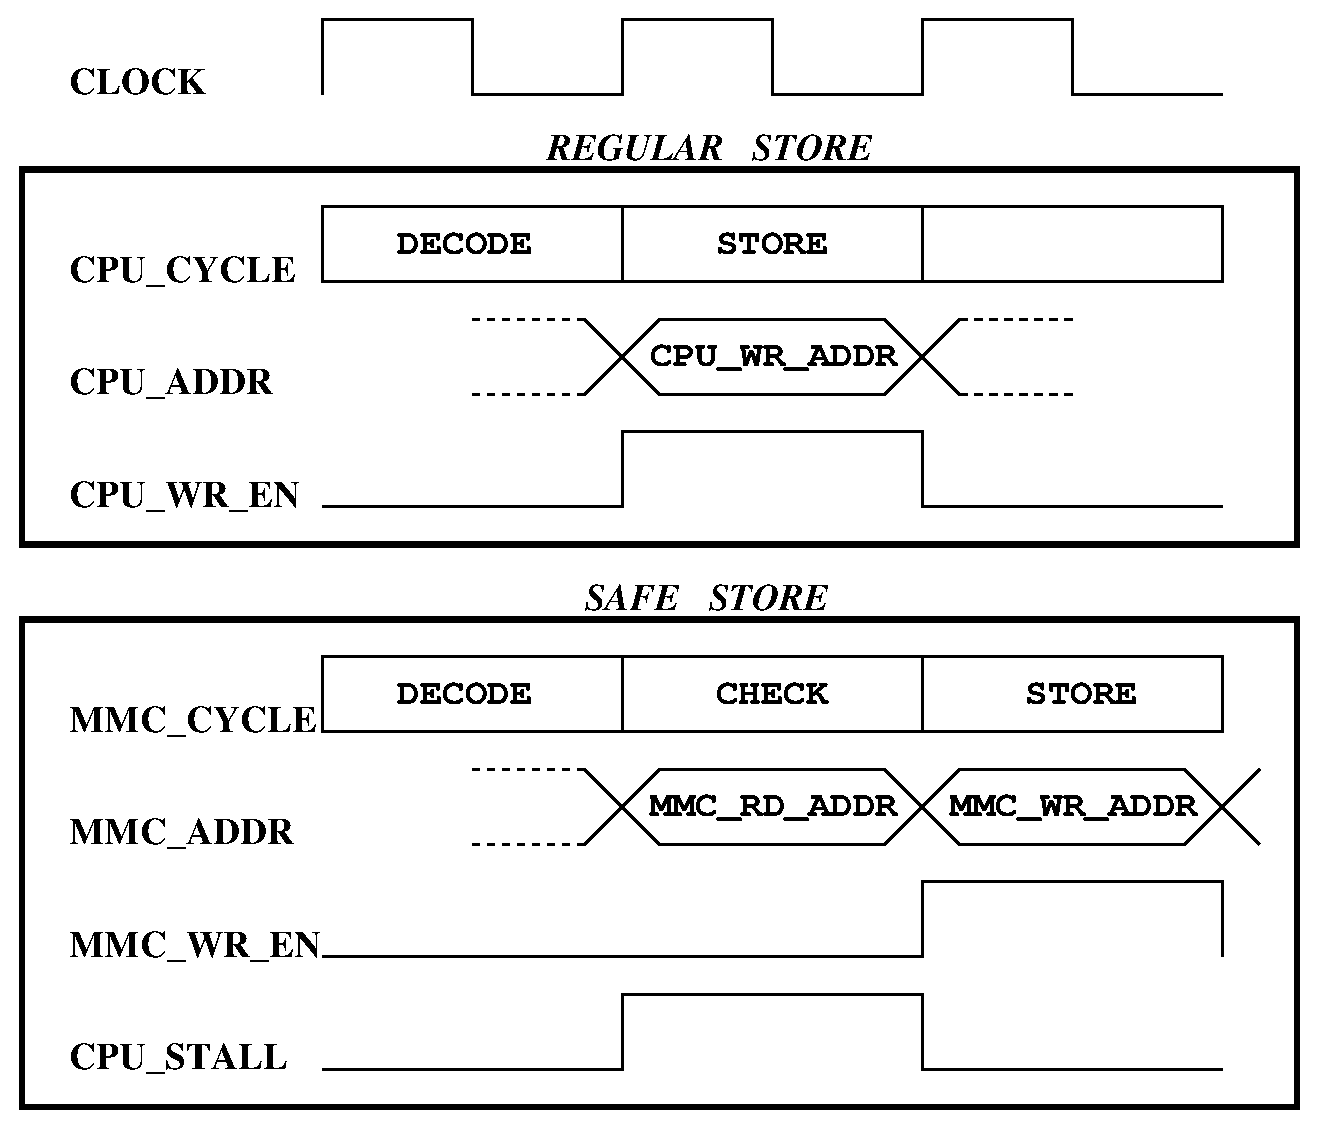
\includegraphics[height=2in,
%    keepaspectratio=true]{figures/mmcop.eps} 
%    \caption{Memory Map Controller (MMC)}
%    \label{fig:mmcop}
% \end{figure}
% %z
%-----------------------------------------------------------------
\subsubsection{MMC Operation}
%
We describe the operation of MMC by explaining the different steps in
the execution of a store instruction.
%
Regular store operation takes two clock cycles on AVR.
%
In the first clock cycle, the instruction is decoded and the data to
be written is read from the register file.
%
The processor issues the write address and the write enable in the
second clock cycle.
%
This is illustrated in Figure~\ref{fig:mmcopst}.
%
In the protected mode, the store operation requires an additional
clock cycle (Figure~\ref{fig:mmcopsafest}).
%
The operation in the first clock cycle is similar to a regular store;
instruction decoding followed by a read of the data to be written from
the register file.
%
In the subsequent clock cycles, the MMC performs three operations.
%
First, it stalls the processor execution and takes control of the
address bus to memory.
%
This occurs in the second cycle of the clock waveform shown in
Figure~\ref{fig:mmcopsafest}.
%
In the same clock cycle it performs an address translation operation
to determine the address of the permissions in the memory map.
%
Address translation is implemented as combinational logic as shown in
Figure~\ref{fig:umpuaddrtans}.
%
Memory map permissions are also read in this cycle as the MMC unit has
control over the address bus.
%
Second, the MMC compares the ownership information to the identity of
the current executing domain.
%
The combinational logic of the checker is shown in
Figure~\ref{fig:umpupermscheck}.
%
Finally, if the check is successful, then the MMC issues a write
enable signal to the data memory; else an \texttt{MMC\_PANIC} signal is
asserted.
%
%
\begin{figure}[htpb]
 \centering
  \mbox{
    \subfigure[Address
    Translation]{\label{fig:umpuaddrtans}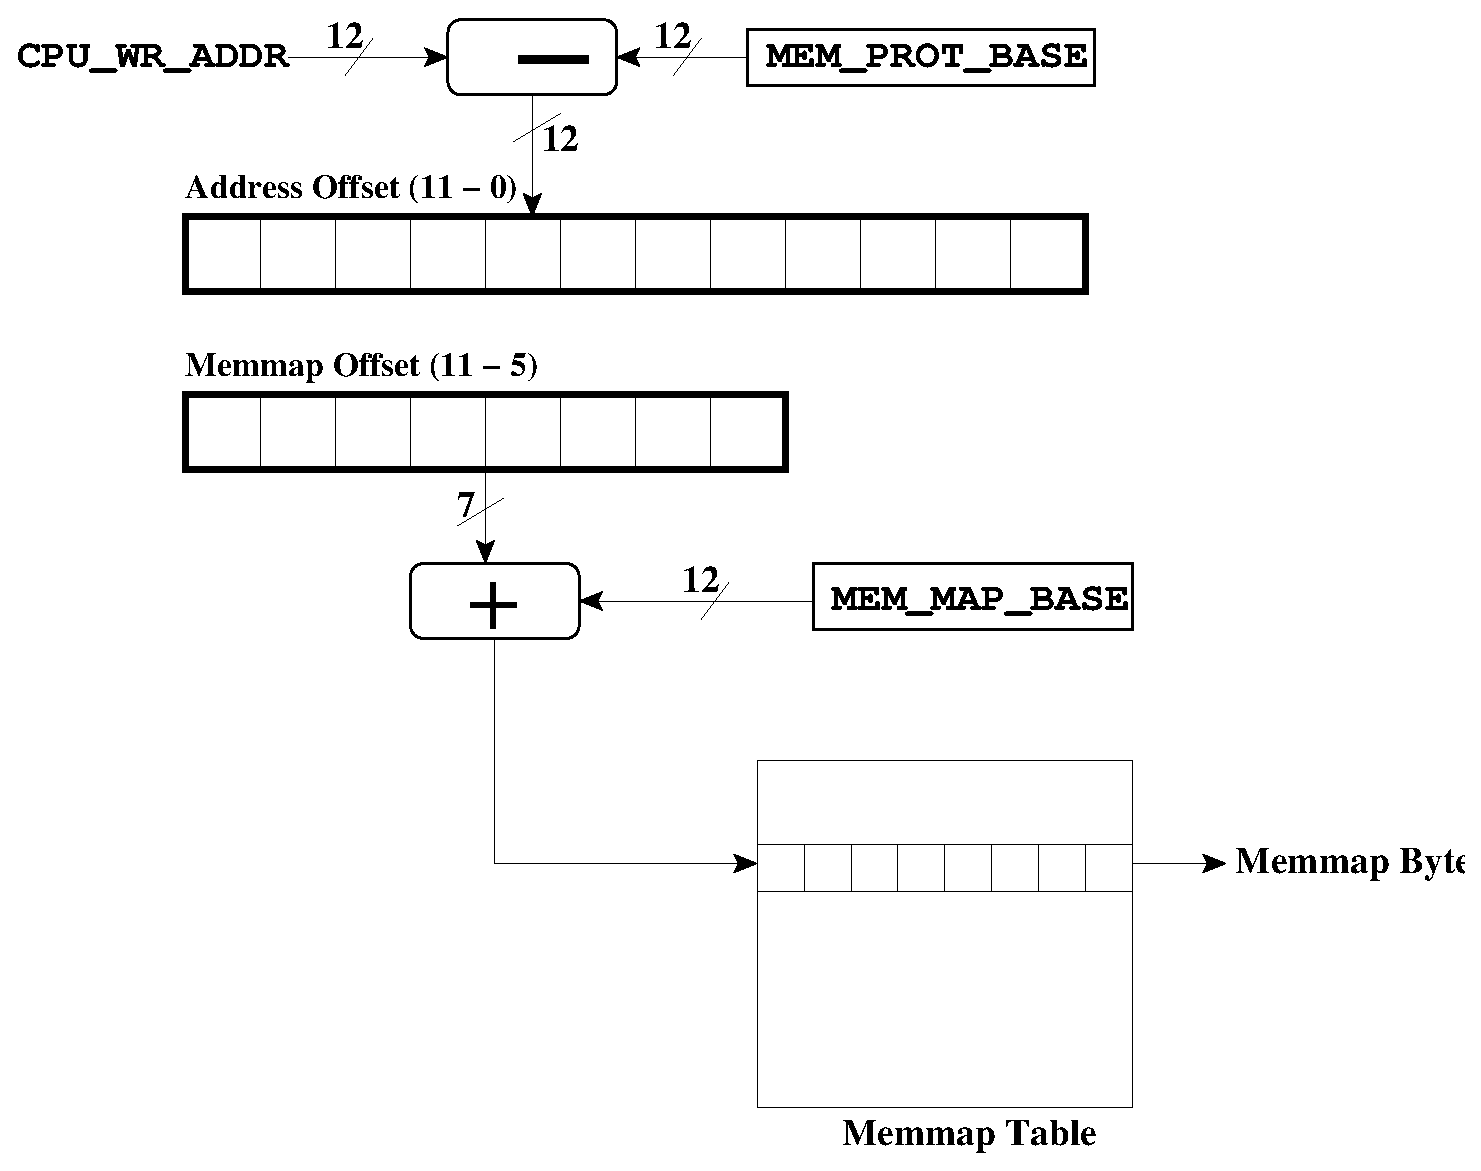
\includegraphics[width=2.5in,
      keepaspectratio = true]{figures/umpuaddrtans.eps}}
    \hspace{0.2in}
    \subfigure[Permission
    Checker]{\label{fig:umpupermscheck}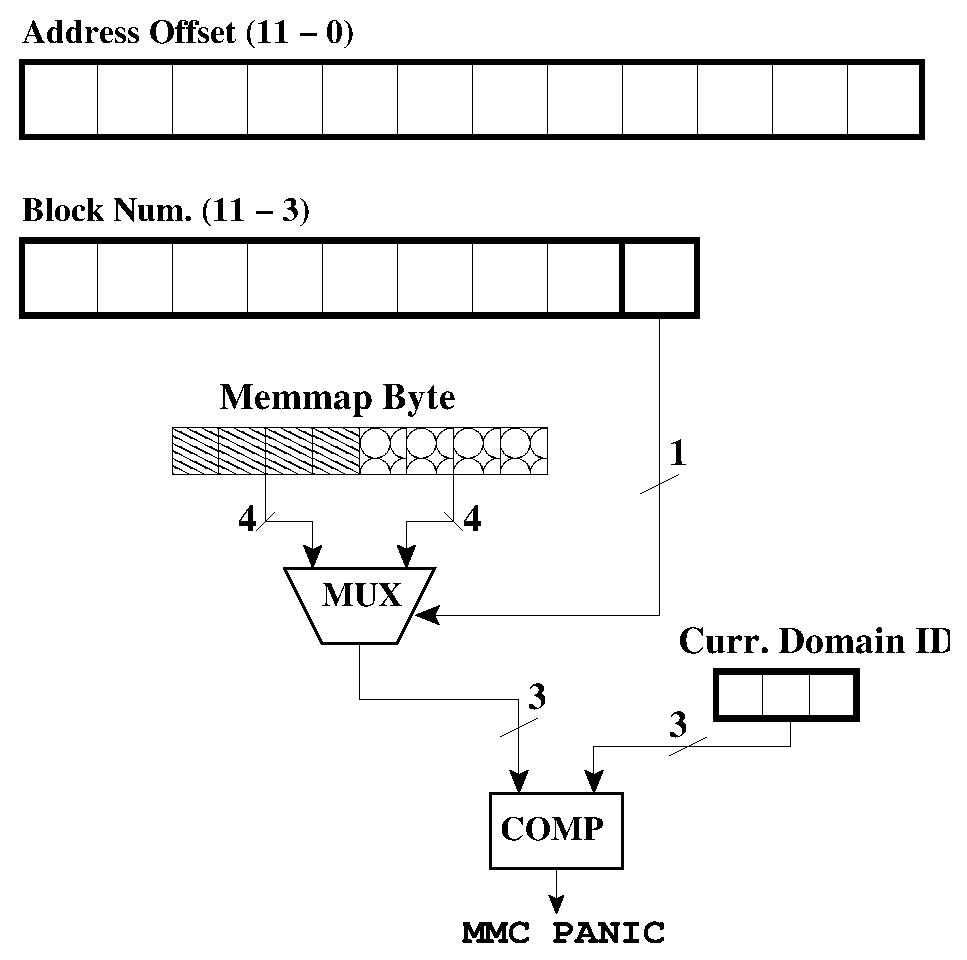
\includegraphics[width=2.5in,
      keepaspectratio = true]{figures/umpupermscheck.eps}}
  }
  \caption{MMC Operations (8-domain)}
\end{figure}   
%
%
%----------------------------------------------
\subsubsection{MMC Software Library}
\label{sec:mmc_for_protection}
%
The software library is responsible for the initialization of MMC.
%
Memory map controller is configurable through a set of
programmable registers shown in Table~\ref{tab:mmap_config_regs}.
%
The registers are accessible only from the trusted domain.
%
The address range to be protected by the memory map is input to the
software library; the library appropriately initializes the registers
\texttt{mem\_prot\_base} and \texttt{mem\_prot\_top}.
%
It provides macros to initialize the \texttt{mem\_map\_config}
register that configures the block size and the number of protection
domains available in the system.
%
Our design is flexible to accommodate different block sizes and number
of domains.
%
\begin{table}[htdp]
\centering
\small{
\begin{tabular}{|l|l|}
	\hline
	Register & Function\\
	\hline
	\texttt{mem\_map\_base} & Memory map base pointer \\
	\texttt{mem\_prot\_base} & Lower bound of protected address space\\
	\texttt{mem\_prot\_top} & Upper bound of protected address space\\
	\texttt{mem\_map\_config} & Configure block size and domains\\
	\hline
\end{tabular}}
\caption{Memory Map Configuration Registers}
\label{tab:mmap_config_regs}
\end{table}

The software library also manages the memory map.
%
It provides custom implementations of the \texttt{malloc},
\texttt{free} and \texttt{change\_own} calls that are carefully
designed to protect against some common programming bugs discussed in
Section~\ref{sec:mmap_for_protection}.
%
A special read-only register contains the identity of the currently
execution domain.
%
This register is tracked and updated by the domain
tracker (Section~\ref{sec:domtracker}).
%
All the APIs in the software library only trust the information stored
in this register.
%
For example, the memory map is updated with the identity stored in
this register during a call to \texttt{malloc}.
%
%------------------------------------------------------------
\subsection{Control Flow Controller}
\label{sec:cfctrl}
%
Control Flow Controller (CFC) ensures that control can never flow out of
a domain, except via calls to functions exported by other domains, and
via returns to calls from other domains.
%
Conversely, control flow can enter a domain only through an exported
function or through the return site of a call that is made to a
function exported by some other domain.
%
%In this section, we describe the different functional units that constitute the Control Flow controller.
%
The CFC comprises of software run-time components, desktop tools and hardware functional units that work together to ensure control flow integrity.
%
The Cross domain linker (Section~\ref{sec:cross_domain_linking}) sets up the domains and the jump table in the program memory.
%
The Cross Domain Call Unit (Section~\ref{sec:cdcunit}) implements the
cross domain call mechanism using the domain tracker
(Section~\ref{sec:domtracker}) and a safe stack
(Section~\ref{sec:umpuss}).

%
The Domain Bounds Checker (Section~\ref{sec:dombndschecker}) ensures that the control flow never leaves a domain except through valid points.
%
This section describes all the components of CFC.
%This section describes the design of CFC components and the linking mechanism used to implement cross domain calls.
%---------------------------------------------------
\subsubsection{Cross Domain Linking}
\label{sec:cross_domain_linking}
%
The set of functions exported by a domain are parsed by a cross domain
linker tool that automatically generates a jump table in the
flash memory.
%
The jump table as described in Section~\ref{sec:crossdomcall}, is
similar in design to the processor interrupt vector table.
%
Each entry in jump table is an instruction to jump to a valid exported
function.
%
Each domain has its own jump table that contains all functions that it
exports. 

The current implementation of the cross domain linker simply parses a
header file that contains all the functions exported by a domain.
%
It then generates a jump table using the symbol names of the exported
functions.
%
All the references to the exported functions are replaced by references to
the corresponding entries in the jump table.
%
The linker can be improved if the programming language contains
semantics that define an interface.
%
An example of such a language that is popular in sensor networks is
NesC~\cite{gay03nesc}.
%-----------------------------------------------------------
\subsubsection{Cross Domain Call Unit}
\label{sec:cdcunit}
%
This section describes the design and implementation of the Cross domain call unit in UMPU.
%
The operations performed during the cross domain call are similar to the Harbor's cross domain call described in Section~\ref{sec:crossdomcall}.
%

A cross domain call is triggered whenever the control flow reaches the jump table through any of the call instructions.
%
As shown in Figure~\ref{fig:cdcinit}, the base address of the jump
table is stored in the UMPU register
\texttt{umpu\_jmp\_tbl\_base\_ptr}.
%
This register is initialized during boot up by the software library.
%
The signals indicating a call instruction and the call address are
provided by the fetch decoder unit in the processor.
%
The combinational logic in the cross domain call unit asserts the \texttt{UMPU\_CDC\_EN} signal.
%
This signal triggers the cross domain call state machine as shown in Figure~\ref{fig:cdcstmc}.
%
The state machine pushes the previous domain ID, stack bounds and cross domain return address onto the safe stack.
%
The new domain ID is updated by the domain tracker.
%
The new stack bounds is determined from the run-time stack pointer.
%
The new cross domain return address is updated by the fetch decoder unit.
%
\begin{figure}[htpb]
 \centering
  \mbox{
    \subfigure[Cross Domain Call Init]{\label{fig:cdcinit}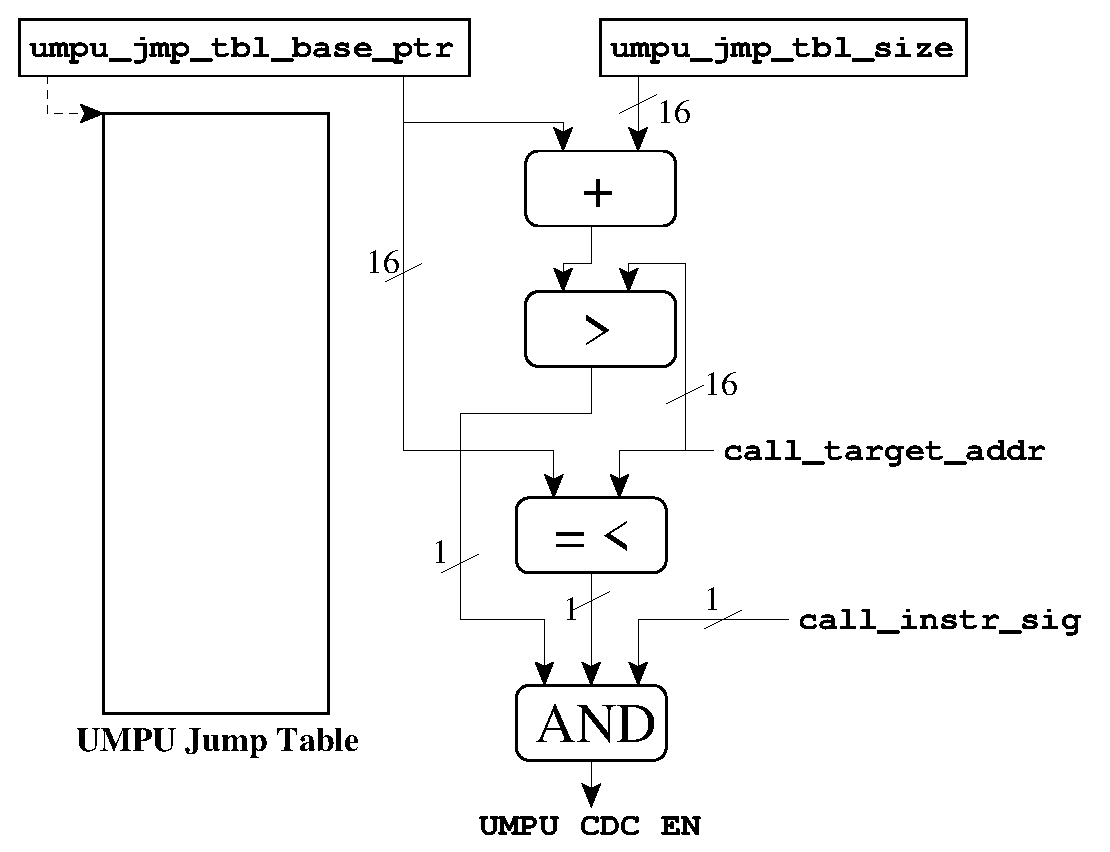
\includegraphics[width=2.5in,
      keepaspectratio = true]{figures/umpucdcinit.eps}}
    \hspace{0.2in}
    \subfigure[Cross Domain Call State Machine]{\label{fig:cdcstmc}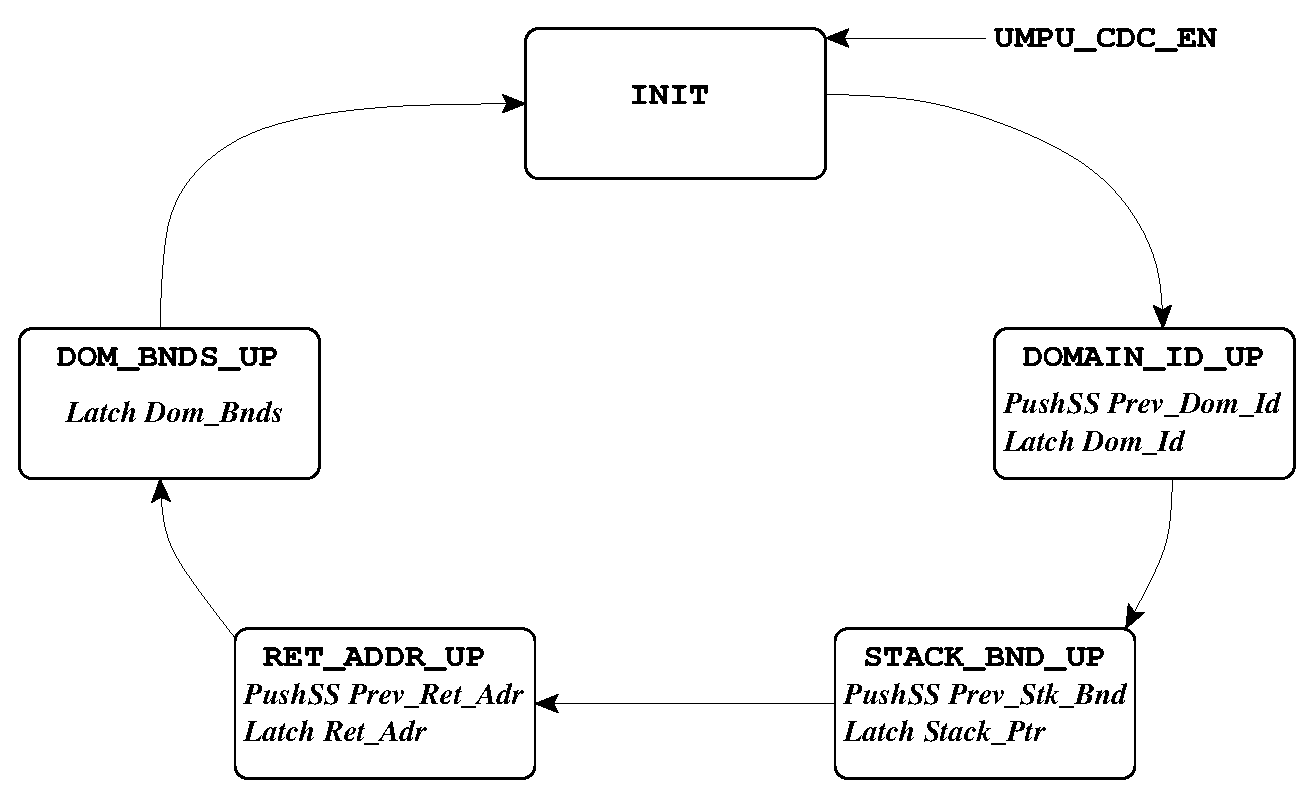
\includegraphics[width=2.5in,
      keepaspectratio = true]{figures/cdcstatemc.eps}}
  }
  \caption{Cross Domain Call Unit}
\end{figure}   

A cross domain return is triggered during the execution of a processor's \texttt{ret} instruction.
%
The signals indicating a \texttt{ret} instruction and the return address are sent to the cross domain call unit by the processor's fetch decoder unit.
%
A cross domain return is initiated if the return address matches the stored cross domain return address.
%
During a cross domain return, the previous values of the domain ID, stack bounds and cross domain return address are restored from the safe stack.
%
The cross domain return is also implemented as a state machine.
%
%---------------------------------------------------
\subsubsection{Domain Tracker}
\label{sec:domtracker}
%
The domain tracker is a functional unit that tracks the execution of
the currently executing domain.
%
The updated domain ID is stored in a special read-only register.
%
The value stored in the register is used by the memory map controller
to validate the access permissions for a store operation.
%
The domain tracker is triggered by the \texttt{UMPU\_CDC\_EN} signal
(Figure~\ref{fig:cdcinit}) or by the occurrence of an interrupt.
%
We discuss interrupts later in Section~\ref{sec:umpuintr}.
%
The jump tables of all the domains are located next to one another in
the program memory.
%
The maximum number of entries in the jump table for a domain is
configured in the \texttt{umpu\_dom\_jmp\_tbl\_size}.
%
Once triggered, the functional unit subtracts the
\texttt{umpu\_jmp\_tbl\_base\_ptr} from the cross domain call address
to determine the offset into the jump table.
%
The offset is divided by the size of a domain's jump table to
determine the new domain ID.
%
The combinational logic implementing the domain tracker is shown in
Figure~\ref{fig:domtracker}.
%
The number of entries is chosen to be a power of 2 to implement the
division operation as a shifter.
%
 \begin{figure}[htbp]
    \centering
    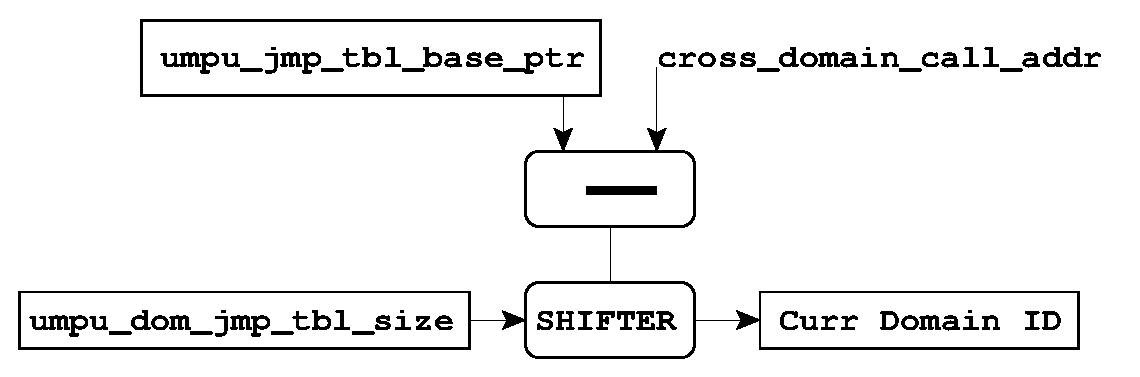
\includegraphics[height=1in,
    keepaspectratio=true]{figures/domtracker.eps} 
    \caption{Domain Tracker}
    \label{fig:domtracker}
 \end{figure}

%---------------------------------------------------
\subsubsection{Safe Stack}
\label{sec:umpuss}
%
UMPU maintains a separate stack in the protected region of memory to
store important state information related to cross domain calls
(Figure~\ref{fig:cdcstmc}).
%
The \texttt{safe\_stack\_ptr} is initialized by the software library
to reside in a protected region of data memory.
%
The hardware does not check whether the safe stack is protected or not.
%
The size of the safe stack is set during initialization.
%
The hardware checks to ensure that there is no overflow of safe stack.
%
%-----------------------------------------------------------
\subsubsection{Domain Bounds Checker}
\label{sec:dombndschecker}
%
The domain bounds checker ensures that the control flow does not leave
a domain except through the jump table.
%
The program memory layout showing different domains, jump table,
interrupt table and the bootloader is shown in
Figure~\ref{fig:progmemlayout}.
%
The program memory address space can be statically partitioned
or it can use a mechanism similar to the SOS module
loader~\cite{ram05sos}.
%
But the end result of either mechanism is that there is no overlap in
the address space of any modules.
%
Based on this assumption, the domain bounds checker comprises of two
components (Figure~\ref{fig:dombndscheck}).
%
First, a \emph{Domain Bounds Table} that stores the lower and upper
address bounds for every domain.
%
Second, a \emph{PC Bounds Checker} implemented as a combinational logic
block which ensures that the program counter always lies within the
bounds of the current domain or in the jump table.
%
\begin{figure}[htbp]
   \centering
   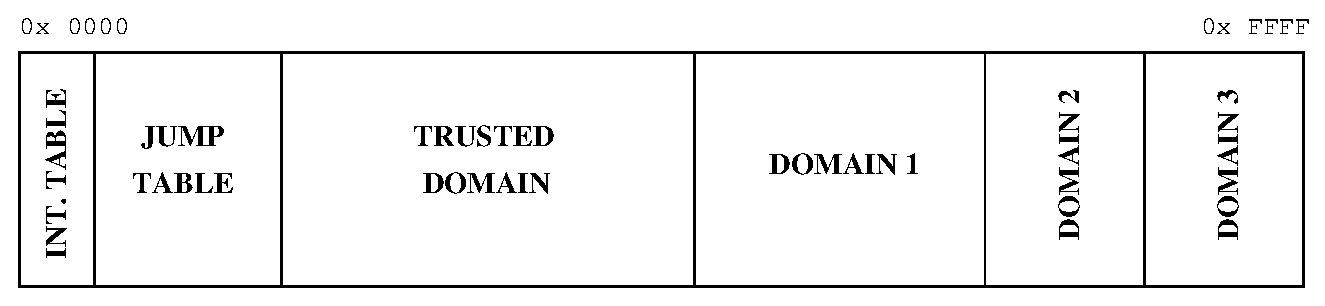
\includegraphics[height=1in,
   keepaspectratio=true]{figures/progmemlayout.eps} 
   \caption{Program Memory Layout}
   \label{fig:progmemlayout}
\end{figure}
\begin{figure}[htbp]
   \centering
   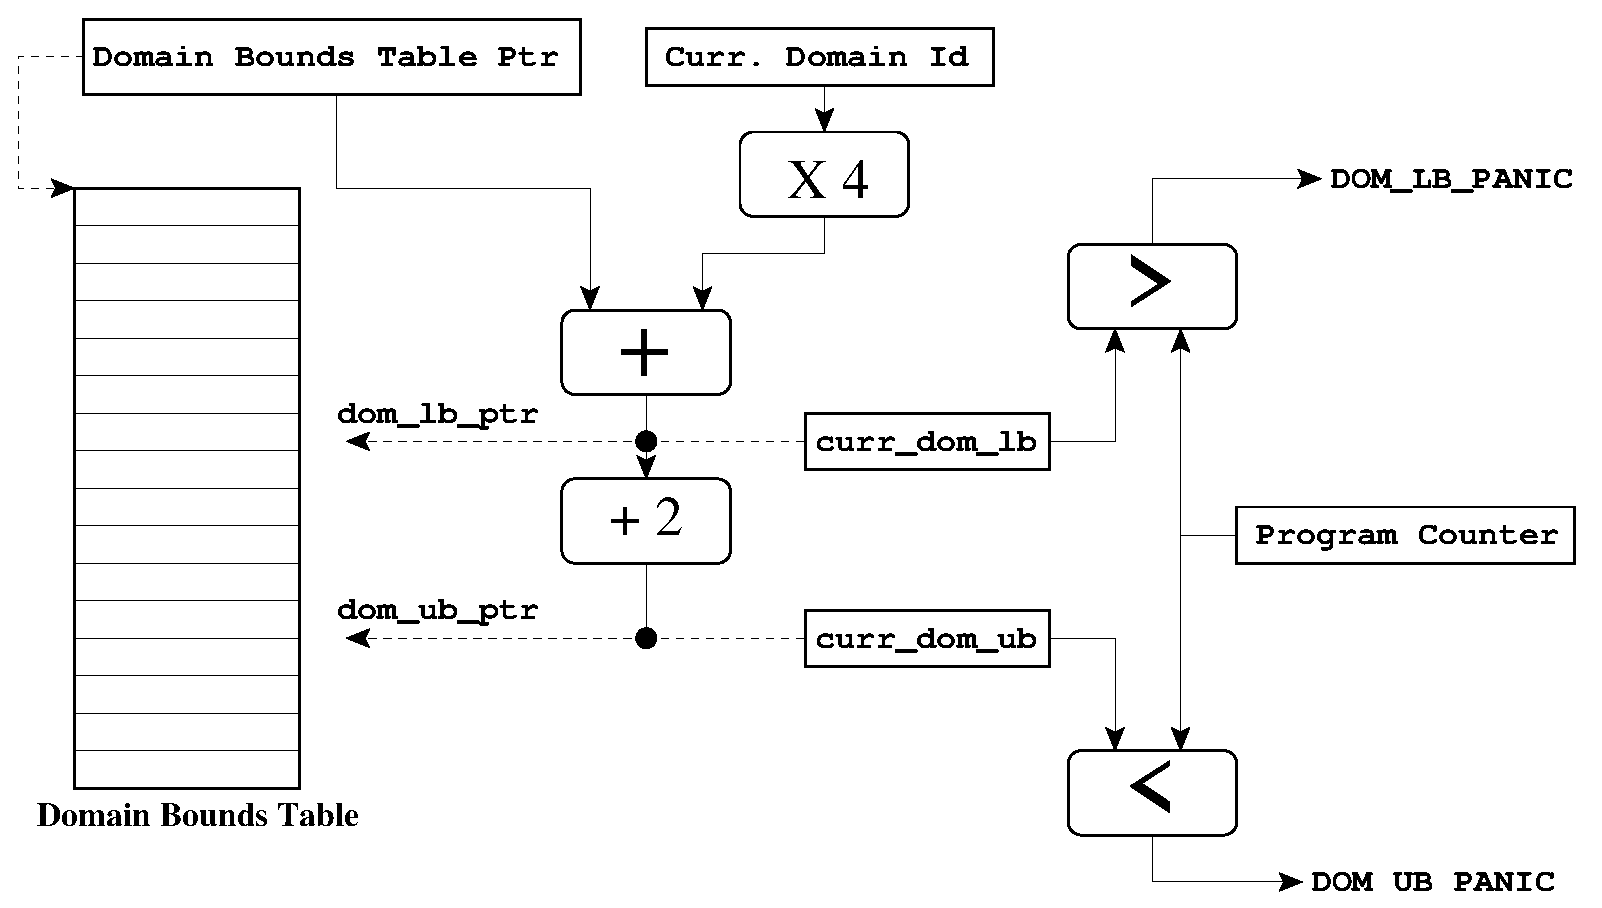
\includegraphics[height=2.5in,
   keepaspectratio=true]{figures/domboundschecker.eps} 
   \caption{Domain Bounds Checker (8 Domains)}
   \label{fig:dombndscheck}
\end{figure}

The domain bounds table can be statically initialized or it
can be filled by a module loader running in the trusted domain.
%
As shown in Figure~\ref{fig:dombndscheck}, the registers
\texttt{dom\_lb\_bnd} and \texttt{dom\_ub\_bnd} store the lower and the
upper bounds of the addresses for the current domain.
%
These registers are updated during every cross domain call.
%
There are two alternate implementations of the domain bounds checker
that have a different performance and area utilization.
%
The domain bounds table can be implemented as a RAM/FLASH based
look-up table or it can be implemented as a register array.
%
The look-up table has more overhead than a register array
implementation because the bounds values for a domain have to be
loaded from memory onto the registers; the bounds can be directly read
from a register array.
%
The register array occupies more area and therefore increases the area
of the processor.
%
We have opted for the register array implementation as it improves the
performance of the system.
%
The PC bounds checker issues a panic signal when the program counter
lies outside the domain bounds.
%
The panic signal is suppressed if the new program counter lies within
the jump table or the interrupt vector table.
%
%------------------------------------------------------------
\subsection{Run-Time Stack Integrity}
\label{sec:umpuruntimestackprot}
%------------------------------------------------
\subsubsection{Stack Bounds Protection}
The run-time stack is protected from cross domain corruption through
the usage of stack bounds.
%
The stack bounds are set by storing the value of the stack pointer
during a cross domain call.
%
The functional unit performs two checks.
%
The first check is an extension to the Memory map controller shown in
Figure~\ref{fig:stackbndscheck}.
%
All store instructions whose address is greater than the current stack
bound and lesser than the run-time stack base address are invalid.
%
\texttt{MMC\_STACK\_PANIC} signal is generated upon an invalid stack
access.
%
The \texttt{stack\_base} register is set to the initial value
of the stack pointer during bootup.
%
The base register is required to allow the stack pointer to be setup
anywhere in the data memory.
%
The second check is to protect against stack underflow within a domain
that could occur due to mismatched push and pops.
%
A \texttt{STACK\_UNDERFLOW\_PANIC} is generated upon error.
%
\begin{figure}[htbp]
  \centering
  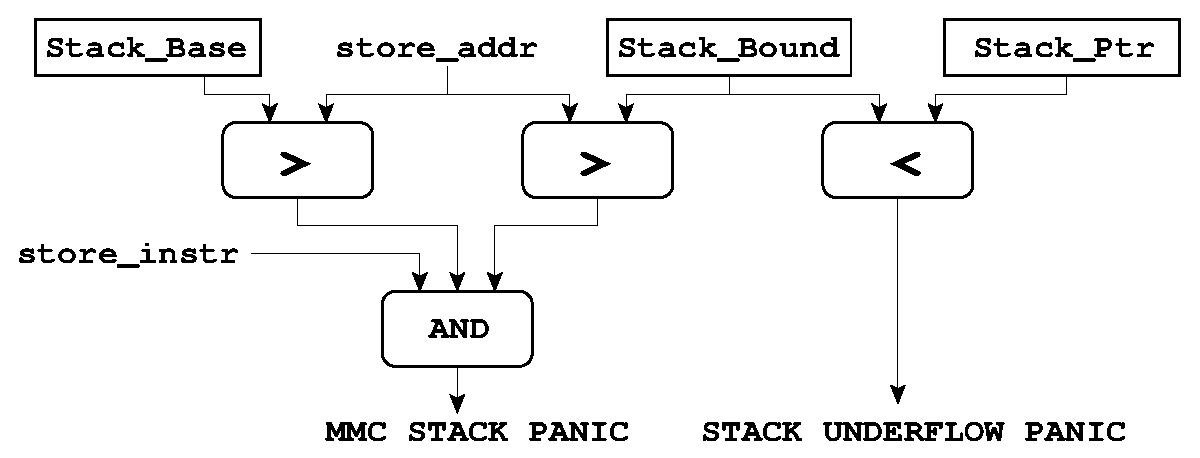
\includegraphics[height=1in,
  keepaspectratio=true]{figures/umpustackprot.eps} 
  \caption{Run-Time Stack Checker}
  \label{fig:stackbndscheck}
\end{figure}
%
%--------------------------------------------
\subsubsection{Stack Overflow Protection}
A simple stack overflow check is also implemented that
triggers a panic when the stack pointer exceeds a pre-initialized
upper bounds.
%-------------------------------------------
\subsubsection{Return Address Protection}
%
The stack bounds protection cannot prevent the corruption to the stack that is internal to the domain.
%
Such corruption can modify the return addresses stored on the run-time stack.
%
Note that the domain bounds checker will detect such a corruption if the return address lies outside the domain bounds.
%
However, the control flow integrity within the domain is not preserved as the return address could be any arbitrary value within the bounds of the domain.
%
UMPU preserves control flow integrity within a domain by copying the return address to the safe stack in the implementation of the call instruction.
%
Correspondingly, the implementation of the return instruction is also modified to use the return address present in the safe stack.
%
Return address protection increases the run-time size of the safe stack.
%
%------------------------------------------------------------
\subsection{Interrupt Handler Unit}
\label{sec:umpuintr}
%
The interrupt handling in the processor is modified to incorporate the
memory protection extensions.
%
In UMPU, by default, all the interrupts are handled in the trusted domain.
%
A verifier running on the desktop scans the interrupt vector table to
ensure that no interrupt handler is located outside the trusted
domain.
%
When the processor begins handling a pending interrupt, it generates a
signal that triggers the UMPU Interrupt Handler Unit.
%
The processor is stalled for a single clock cycle by the Interrupt
Handler Unit and the domain tracker is signaled to update the current
domain ID to the trusted domain.
%
The previous domain ID is pushed onto the safe stack.
%
Thereafter, the control flow within the interrupt handler proceeds as
normal.
%
There are no checks during the execution of the handler in the trusted
domain.
%
But cross domain calls in the interrupt handler can transfer control
to the other domains.
%
Therefore, all the domains can process the interrupts despite their
origin in the trusted domain.
%

All processors have a special \texttt{reti} instruction to return from
the interrupt and resume normal execution.
%
UMPU modifies the implementation of \texttt{reti} to include an extra
clock cycle to restore the domain ID of the interrupted domain from
the safe stack.
%
In addition, UMPU disallows the execution of the \texttt{reti} instruction from the non-trusted domain.

An alternate design is to register an interrupt with any
domain.
%
The registration information is stored along with the interrupt
vector table.
%
This allows the processor to directly transfer control to the registered domain
upon receiving an interrupt.
%
This design will have a lower overhead but will incur the cost of a
registration table in FLASH/RAM.
%------------------------------------------------------------
\subsection{UMPU Exception Controller}
%
We have implemented an exception mechanism in UMPU to allow the
embedded software to perform suitable recovery in the event of a panic
condition.
%
The UMPU Exception Controller monitors all the panic signals that can
be generated by the various UMPU extensions.
%
Whenever, any panic signal goes high, it generates an interrupt
condition.
%
The interrupt is set to have the highest priority.
%
Further, the interrupt is set to be non-maskable that guarantees its
delivery under all conditions.
%
The Controller also stores some information relating to the exception
that enables the design of recovery routines.
%
For example, the Controller stores the cause of the exception, the
program counter at which the exception occurs and the stack pointer.
%
Table~\ref{tab:umpuexceptions} contains the UMPU exception signals and
the conditions that trigger them.
%
\begin{table}[htdp]
\centering
\small{
\begin{tabular}{|l|l|}
	\hline
	Signal & Condition\\
	\hline
	\texttt{MMC\_PANIC} & Memory map permission violation
        (Fig.~\ref{fig:umpupermscheck})\\
	\texttt{MMC\_STACK\_PANIC} & Run-time stack bounds violation
        (Fig.~\ref{fig:stackbndscheck})\\
	\texttt{STACK\_UNDERFLOW\_PANIC} & Stack pointer lower than
        the stack bound (Fig.~\ref{fig:stackbndscheck}) \\
	\texttt{STACK\_OVERFLOW\_PANIC} & Stack overflow violation
        (Sec.~\ref{sec:umpuruntimestackprot})\\
        \texttt{DOM\_LB\_PANIC} & Control flow outside domain lower
        bound (Fig.~\ref{fig:dombndscheck})\\
        \texttt{DOM\_UB\_PANIC} & Control flow outside domain upper
        bound (Fig.~\ref{fig:dombndscheck})\\
	\hline
\end{tabular}}
\caption{UMPU Exception Signals and Conditions}
\label{tab:umpuexceptions}
\end{table}

%------------------------------------------------------------
\subsection{Configurable Soft-Core}
%
The UMPU extensions have been designed with a lot of flexibility that
enables them to be configurable by software at run-time.
%
For example, the block size used in the memory map can be set by
the software in the trusted domain during initialization.
%
This adds complexity to the design of the UMPU extensions as the
functional units have to be designed to accommodate inputs of arbitrary
length.
%
An instance of such a functional unit is a variable length shifter that
needs to be introduced to support the address translation operations.
%
There are many similar examples in the other UMPU extensions as well.

An alternative is to implement the UMPU extensions as configurable
soft-cores.
%
The configurable soft-cores have the benefit of reduced hardware
complexity but they also lose the run-time flexibility.
%
The soft-core is ideally suited for application specific
system-on-chip (SoC) designs where the protection requirements can be
determined apriori.




















%%%%%%%%%%%%%%%%%%%%
% EVALUATION
%%%%%%%%%%%%%%%%%%%%
\section{Evaluation}
\label{sec:eval} 
%
In this section, we analyze the protection benefits and overheads
introduced by Harbor memory protection mechanisms.
%
We first present microbenchmarks that measure Harbor's CPU overhead
and resource utilization for a software-only implementation.
%
We follow that with a similar evaluation for UMPU.
%
Later, we compare the application level performance in the presence of
various protection mechanisms.
%
We conclude this section with a discussion on the various programming
errors that can be detected and prevented by Harbor memory protection.
%
%--------------------------------------------------------------
\subsection{Harbor CPU Overhead Microbenchmarks}
%
We first present microbenchmarks that measure Harbor's CPU overhead.
%
Overhead was measured using Avrora~\cite{titzer05avrora}, a cycle
accurate node and network simulator for the Mica family of sensor
nodes.
%
Measurements were averaged across multiple application scenarios.
%
%--------------------------------------------------------------
\subsubsection{Overhead of Harbor Primitives}
%
Table~\ref{tab:harbor_routines} summarizes the results for all of Harbor's
protection primitives.
%
All these routines are implemented in assembly for optimizing performance.
%
The registers used in these routines are saved to the run-time stack.
%
Many CPU cycles are spent in push and pop operations.
%
This overhead could be significantly reduced by dedicating one or more
registers for Harbor's exclusive use; the cross-compiler would be directed
to ignore these registers entirely.
%
%% The cross compiler can be directed to produce binary that does not use few registers.
%% %
%% The registers left unused by compiler can be used freely in memory protection assembly routines without saving them to stack.
%
However, \texttt{avr-gcc} does not have stable support for dedicated registers.
%

\begin{table}[htdp]
\centering
\small{
\begin{tabular}{|l|c|}
	\hline
	Function Name & Cost\\
	\hline
	\texttt{write\_access\_check} & 65~cyc\\
	\texttt{cross\_domain\_call} & 65~cyc\\
	\texttt{cross\_domain\_return} & 28~cyc\\
	\texttt{func\_entry\_stub} & 38~cyc\\
	\texttt{func\_exit\_stub} & 38~cyc\\
	\hline
\end{tabular}}
\caption{CPU Overhead of Memory Protection Routines}
\label{tab:harbor_routines}
\end{table}

Our implementation of some of the \texttt{cross\_domain\_call} and
\texttt{cross\_domain\_return} assumes that the modules follow the
\texttt{avr-gcc} ABI.
%
This optimizes the performance of these routines as they are free to use
the caller used registers defined in the ABI.
%
In addition, these routines can also use the scratch registers.
%
This results in a total of six registers that can be used by in the
AVR architecture (\texttt{R0, R1, R26, R7, R30 and R31}).
%
However, the implementation of the \texttt{function\_entry\_stub} and
\texttt{function\_exit\_stub} cannot use the caller-used registers
because some of the compiler inserted routines for integer arithmetic
do not follow the regular calling conventions.
%--------------------------------------------------------------
\subsubsection{Memory Map Overhead}
%
Overhead is also introduced during dynamic memory allocation, deallocation,
and transfer, since the memory map must be updated.
%
Table~\ref{tab:malloc_comparison} compares the overhead of memory
allocation routines in the presence and absence of the protection
mechanism.
%
The overhead depends upon the size of memory block that is being
allocated, freed or transferred.
%
The average size of the memory block used by all the three operations in
our experiments was 16 bytes.
%
The numbers in Table~\ref{tab:malloc_comparison} are an average
measurement of the execution time obtained from a long running
simulation of the Surge application~\cite{woo03surge}.
%
The relatively higher overhead of \verb+ker_change_own+ and \verb+ker_free+
calls is due to additional checks introduced to prevent illegal
ownership transfer or freeing of memory blocks by non-owners.
%
\begin{table}[htdp]
\centering
\small{
\begin{tabular}{|l|c|c|}
	\hline
	Function Name & Normal & Protected \\
	\hline
	\texttt{ker\char`\_malloc}  & 343~cyc & 610~cyc \\
	\texttt{ker\char`\_free} & 138~cyc & 425~cyc\\
	\texttt{ker\char`\_change\char`\_own} & \hphantom{0}55~cyc & 365~cyc \\
	\hline
\end{tabular}}
\caption{CPU Overhead for Dynamic Memory Calls}
\label{tab:malloc_comparison}
\end{table}
%
%--------------------------------------------------------------
\subsection{Harbor Resource Utilization Microbenchmarks}
%--------------------------------------------------------------
\subsubsection{Resource Utilization of Harbor Primitives}
%
Increases in code and data memory utilization due to Harbor's
protection mechanisms are shown in
Table~\ref{tab:kernel_size_comparison}.
%
Code memory usage increases by about 15\% in a protected kernel
relative to an unprotected kernel.
%
This increase is mainly due to the memory map and cross domain call
jump table mechanisms.
%
There is no significant change in program memory usage going from two
protection domains to multiple protection domains.
%
Data memory usage increases relative to an unprotected kernel by at
most 5\% and 9.5\% in 2-domain and 8-domain systems, respectively.
%
The main culprit is the memory map, which takes 128 and 256~bytes in 2-
and 8-domain systems.  (There are 28~additional bytes of constant
overhead.)
%
This is the maximum possible overhead, as this memory map configuration
stores layout and ownership information for the entire address space.
%
%% Memory map sizes are 128 bytes and 256 bytes respectively for
%% two-domain and multi-domain configurations.
%
By modifying data layout, the portion of address space that requires a
memory map can be reduced.
%
For example, in SOS, memory map is needed only for the heap and the safe
stack; by abutting these data structures, the memory map can be
reduced to 70 or 140~bytes for 2- and 8-domain protection, respectively.
%
%% By abutting these two data-structures, size of memory map required can be reduced to 70 bytes for two-domain protection (140 bytes for multi-domain protection)\footnote{There is 28 byte constant overhead. Therefore total overhead is 98 bytes}.
%
\begin{table}[htdp]
\centering
\small{\def\X{\hphantom{0}}
\begin{tabular}{|l|c|c|c|c|c|}
	\hline
	Memory & Raw & \multicolumn{2}{c|}{$\Delta$ (2 domains)} & \multicolumn{2}{c|}{$\Delta$ (8 domains)}
	\\
	\hline
	Flash\raise1pt\hbox{\strut}  & 41796 B & +6146 B & +14.7\% & +6228 B & +14.9\% \\
	RAM (Max) & \X{}2892 B & \X{}+148 B & \X{}+5.1\% & \X{}+276 B &
	\X{}+9.5\% \\
	RAM (Min) & \X{}2892 B & \X{}\X{}+98 B & \X{}+3.4\% & \X{}+168 B &
	\X{}+5.8\% \\
	\hline
\end{tabular}}
\caption{Code and Memory Overhead for Blank SOS Kernel for Mica2}
\label{tab:kernel_size_comparison}
\end{table}
%------------------------------------------------------------
\begin{table}[htdp]
\centering
\small{\def\X{\hphantom{0}}\def\XX{\X\X}
\begin{tabular}{|l|c|c|c|}
	\hline
	Module & Raw & \multicolumn{2}{c|}{$\Delta$ (2 or 8 domains)} \\
	\hline
	Blink\raise1pt\hbox{\strut} & \XX{}150 B & \XX{}+48 B & +32\%\\
		% 150B -> 198B
	Tree Routing & \X{}2820 B & +1658 B & +59\%\\
		% 2820B -> 4478B
	Surge & \XX{}542 B & \X{}+350 B & +65\%\\
		% 542B -> 892B
	Outlier Det. & \X{}1312 B & \X{}+738 B & +56\% \\
		% 1312B -> 2050B
	DVM & 13072 B & +6652 B & +51\%\\
		% 13072B -> 19724B
	FFT & \X{}3016 B & \X{}+894 B & +30\% \\
		% 3016B -> 3910B
	\hline
\end{tabular}}
\caption{Code Size Increase of Mica2 SOS Modules}
\label{tab:module_size_comparison}
\end{table}

\subsubsection{Size overhead of Sandboxing Modules}
%
Finally, we evaluate the relative increase in size of modules due to
introduction of checks by the binary rewriter.
%
As noted in Table~\ref{tab:module_size_comparison}, there is a significant
increase in the relative code size of sandboxed binaries as compared to raw
binaries.
%
This is mainly caused due rewriting all store instructions to a long
sequence of instructions that call the memory map checker
(Figure~\ref{fig:inlinechecks}).
% 
This overhead could be significantly reduced by using dedicated registers
to eliminate all push/pop instructions in the sequence, and/or by adding
static analysis to eliminate some redundant checks.
%
%
%---------------------------------------------------------------------------
\subsection{UMPU CPU Overhead Microbenchmarks}
%
In this section, we evaluate the CPU overhead of UMPU primitives.
%
We have implemented the hardware components of UMPU by extending
the architecture of the AVR ATMEGA103
microcontroller~\cite{avr103manual}~\cite{avropencores}.
%
The VHDL model of the processor is fully synthesizable.
%
We have instantiated the processor on Xilinx Vertex 2 Pro XC2VP30 FPGA.
%
Our performance overheads are measured using Modelsim 6.0
simulator~\cite{modelsim}.
%
The software library and applications were compiled using
\texttt{avr-gcc} cross compiler.
%
Table~\ref{tab:umpumicrobmperf} contains the CPU overhead of the UMPU
primitives.
%
A comparison to Harbor's software based implementation
(Table~\ref{tab:harbor_routines}) clearly indicates the superior
run-time performance of the primitives implemented in hardware.
%
\begin{table}[htdp]
\centering
\small{
\begin{tabular}{|l|l|c|}
	\hline
	UMPU Function Unit & Function Name & Cost\\
	\hline
	Memory Map Controller &\texttt{write\_access\_check} & 1~cyc\\
	Cross Domain Call Unit &\texttt{cross\_domain\_call} & 5~cyc\\
	Cross Domain Ret. Unit &\texttt{cross\_domain\_return} & 5~cyc\\
	Safe Stack Unit &\texttt{func\_entry\_stub} & 0~cyc\\
	Safe Stack Unit &\texttt{func\_exit\_stub} & 0~cyc\\
	\hline
\end{tabular}}
\caption{Overhead of UMPU Primitives}
\label{tab:umpumicrobmperf}
\end{table}
%

The \texttt{write\_access\_check} implemented by the memory map
controller requires one clock cycle to read the appropriate memory map
byte from RAM.
%
The address translation operation and the permission checking is
implemented by combinational logic units that do not introduce any overhead.
%

Cross domain call and return have an overhead of five clock cycles
when implemented in hardware.
%
The overhead occurs because the current domain identity, stack bound
and return address have to be pushed to the safe stack before they can
be updated with new values.
%
The total information that needs to be pushed to the stack is five
bytes and only one byte can be written every clock cycle.
%
Similarly on the cross domain return, the five clock cycles are
expended in restoring the values read from the safe stack.

Saving and restoring return addresses to the safe stack does not
introduce any added overhead.
%
This is because the hardware unit for safe stack simply takes over the
address bus when the processor is pushing the return address to the
run-time stack.
%
By stealing the address bus from the processor, the hardware unit is
able to simply redirect the store of the return addresses to the safe
stack.

The memory map software library in UMPU is identical in functionality
and implementation to the Harbor memory map API.
%
Therefore, the CPU overhead of the memory management functions (\texttt{malloc},
\texttt{free} and \texttt{change\_own}) is same as the corresponding
Harbor's functions (Table~\ref{tab:malloc_comparison}).
%
%---------------------------------------------------------------------------
\subsection{UMPU Resource Utilization}
%
The UMPU resource utilization comprises of the increased gate count
due to the hardware extensions and the FLASH and RAM utilization of
the software library.
%
In this section, we are primarily concerned only with the gate count
and area.
%
The FLASH and RAM utilization of the software library in UMPU is
similar to Harbor (Table~\ref{tab:kernel_size_comparison}).



%
We measured the gate count of the UMPU components using the Xilinx ISE
8.2i~\cite{xilinxlink} design and synthesis tools.
%
Table~\ref{tab:umpuarea} summarizes the area overhead of UMPU extensions.
% 
\begin{table}[htdp]
\centering
\small{\def\X{\hphantom{0}}\def\XX{\X\X}\def\XXX{\XX\X}\def\Y{\raise1pt\hbox{\strut}}
\begin{tabular}{|l|c|c|c|c|}
	\hline
	Component & Raw & \multicolumn{2}{c|}{$\Delta$ (2 or 8 domains)} & Fraction \\
	\hline
	AVR Core   & \XX{}16419 Gates &   +10504 Gates & +64.00\% &\XX{}0.4\%\\
	Data Mem.  & \X{}131099 Gates & \XXX{}+0 Gates &  +0.00\% &\XX{}3.0\%\\
        Prog Mem.  &    4195531 Gates & \XXX{}+0 Gates &  +0.00\% & \X{}96.5\%\\
        AVR Total  &    4349691 Gates &   +10504 Gates &  +0.24\% &   100.0\%\\   
	\hline
\end{tabular}}
\caption{Area Increase of UMPU}
\label{tab:umpuarea}
\end{table}

The area of the chip is measured in terms of the number of equivalent
logical gates.
%
The UMPU components residing within the core of the chip increase its
area by 64\%.
%
However, the core occupies only 0.4\% of the total chip area; a very
small fraction.
%
Therefore, the total increase in the area of the chip is only 0.24\%.
%
The Xilinx Vertex FPGA used to synthesize the processor does not have
Flash memory which is typically used to implement program memory.
%
Therefore, the program memory mapped to SRAM block cells occupies a
disproportionately large fraction (96.5\%) of the overall chip area.
%

We estimate the increase in the fraction of area occupied by the CPU
core in a typical sensor node processor after the introduction of the
protection mechanisms.
%
The Spec node~\cite{jasonhillthesis}, is a single chip implementation
of a sensor node comprising of a RISC CPU core, SRAM, 900 MHz RF
Transceiver, collection of communication hardware accelerators and an
analog-digital converter.
%
The RISC CPU core used in Spec is similar to the AVR core comprising
of 8-bit datapath and 16-bit instructions.
%
It also has 32 8-bit general purpose registers.
%
The area of the CPU core and ALU in Spec is 0.3920 mm$^2$.
%
Incorporating the UMPU extensions would increase this area by 0.2501
mm$^2$ to 0.6429 mm$^2$ (assuming an identical area overhead of 64\%).
%
The total die area of the Spec node is 6.25 mm$^2$.
%
Therefore, the fraction of die area occupied by the CPU core will
increase from 6.27\% to 10.28\% in the Spec node equipped with UMPU
extensions (Figure~\ref{fig:dieareacmp}).
%
This is a negligible increase in the fraction of area occupied.
%
The packing efficiency of logic in a chip is never 100\%.
%
Therefore, the UMPU extensions can be accommodated without any increase
to the chip die area.
%
\begin{figure}[htbp]
  \centering
   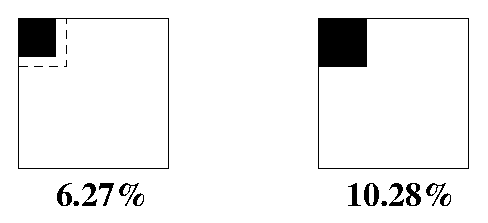
\includegraphics[height = 1.15in, keepaspectratio=true]{figures/areacomp.eps} 
   \caption{Area overhead comparison}
   \label{fig:dieareacmp}
\end{figure}

%
We next measure the fraction of the total increase in the gate count
due to the various UMPU components (Table~\ref{tab:umpuareacomp}).
%
\begin{table}[htdp]
\centering
\tiny{\def\X{\hphantom{0}}\def\XX{\X\X}\def\XXX{\XX\X}\def\Y{\raise1pt\hbox{\strut}}
\begin{tabular}{|l|c|c|}
	\hline
        \hline
	\textbf{Function Unit} & \textbf{Area} & \textbf{Fraction}\\
	\hline
        \hline
        Fetch Decoder Modifications & \XX{}272~Gates & \XX{}2.6\%\\
        \hline
	Memory Map Controller Config. & \XX{}870~Gates & \XX{}8.3\%\\
        \hline
        Memory Map Addr. Trans.       & \XX{}687~Gates & \XX{}6.5\%\\
        \hline
        Memory Map Perms Checker & \XX{}783~Gates& \XX{}7.5\%\\
        Run-Time Stack Checker & & \\
        \hline
        Safe Stack & \X{}2188~Gates & \X{}20.8\%\\
        Cross Domain Call \& Ret State m/c & &\\
	\hline
        Domain Tracker & \X{}1363~Gates & \X{}13.0\%\\
        Cross Domain Call Trig. &&\\
        \hline
        Domain Bounds Checker & \X{}3160~Gates & \X{}30.0\%\\
        \hline
        Exception Generator & \XXX{}31~Gates & \XX{}0.3\%\\
        \hline
        Ram Bus Arbiter & \XX{}390~Gates & \XX{}3.7\%\\
        \hline
        Interrupt Controller Modifications & \XX{}760~Gates & \XX{}7.2\%\\
        \hline
        \hline
        \textbf{Total} & \textbf{10504~Gates} & \textbf{100\%}\\
        \hline
        \hline
\end{tabular}}
\caption{Area breakup of UMPU extensions}
\label{tab:umpuareacomp}
\end{table}

%
The maximum increase in the area occurs due to the Domain Bounds
Checker.
%
We store the domain bounds in a register file to improve the
performance of UMPU during cross domain calls and returns.
%
If area is a primary concern, then the domain bounds can be stored in
a look-up table within RAM or FLASH (Section~\ref{sec:dombndschecker})
%
%--------------------------------------------------------------------------
\subsection{Relative Application Performance}
%
In this section, we measure Harbor performance impact on
applications.
%
We also compare the performance of the software only implementation of
protection with the hardware accelerated UMPU extensions.
%
%----------------------------------------
\subsubsection{Fast Fourier Transform}
%
Many sensor network applications are heavily duty-cycled and therefore
not CPU intensive.
%
However, some are not~\cite{ben06vango}, and for our first benchmark,
we choose a CPU intensive Fast Fourier Transform (FFT).  
%
This should present a realistic idea of Harbor's
costs for challenging applications.
%
The FFT module receives a buffer of 64 samples represented as 16-bit
fixed-point integers (we do not measure the cycles required to obtain the
samples).
%
It transforms the samples in place and outputs results to the same buffer.
%
As shown in Table~\ref{tab:perf_comp}, FFT running on ATMEGA128 (Mica2
sensor node) takes 3.63~ms to execute in normal mode and 17.28~ms in the
protected mode.
%
This gives Harbor a slowdown factor of 4.76.
%
FFT running ATMEGA103 takes 8.24~ms to execute.
%
The execution time of FFT on ATMEGA103 is about two times slower than
on ATMEGA128.
%
This is primarily due to enhanced instruction set of ATMEGA128 which
in particular supports hardware accelerated 8 bit multiplication.
%
FFT routine contains a lot of multiplication operations.
%
The execution of FFT with UMPU protection takes 8.41~ms; a slowdown
factor of only 1.02.
%
In other words, the relative overhead of a computationally intensive
FFT operation with UMPU is only 2\%.
%
%----------------------------------------
\subsubsection{Outlier Detector}
The next experiment is another challenging application, an outlier detector.
%
The outlier detector samples a set of sensor values and stores them in a buffer.
%
Once the buffer is filled, it computes the distance between all pairs of samples in the buffer and stores the result in a matrix.
%
Using a distance threshold, the algorithm marks the distance measurements in the matrix that are greater than the threshold.
%
If the majority of the distance measurements for a sensor readings are marked, then the sensor reading is classified as an outlier.
% %%% <------------- Need Reference !!
%This algorithm is currently being used in the Rate-Adaptive Time Synchronization system.
%
This application is memory write intensive and the matrix operations are easily prone to buffer overflow errors.
%

\begin{table}[htdp]
\centering
\small{\def\X{\hphantom{0}}\def\XX{\X\X}\def\XXX{\XX\X}\def\Y{\raise1pt\hbox{\strut}}
\begin{tabular}{|l|c|c|}
	\hline
	Module & Time (ms) & Slowdown\\
	\hline
	FFT-ATMEGA128\Y		& \XX{}3.63\X & --- \\
        FFT-ATMEGA103\Y         & \XX{}8.24\X & --- \\
        FFT-UMPU                & \XX{}8.41\X & \XXX{}1.02 \\
	FFT-Harbor		& \X{}17.28\X & \XXX{}4.76 \\
	\hline
	Outlier-ATMEGA128\Y	& \XX{}0.18\X & --- \\
        Outlier-ATMEGA103\Y     & \XX{}0.34\X & --- \\
        Outlier-UMPU            & \XX{}0.36\X & \XXX{}1.06\\
	Outlier-Harbor		& \XX{}1.47\X & \XXX{}7.94 \\
	Outlier-DVM		& 102.47\X & \X{}554.50 \\
	Outlier-DVM-Harbor	& 268.32\X & 1452.72 \\
	\hline
	\multicolumn{2}{|l|}{Sort with Mat\'e VM script~\cite{asvm05nsdi}\Y} & \X{}115\hphantom{.0} \\
	\hline
\end{tabular}
}
\caption{Relative Performance of Applications}
\label{tab:perf_comp}
\end{table}

We consider three systems that can protect against such errors,
%
Harbor, UMPU and the Dynamic Virtual Machine (DVM)~\cite{balani06dvm}, an extensible
domain-specific interpreter that performs a bounds check on every write.
%
DVM's bounds checks are in some ways more stringent than Harbor's
protection, since they also prevent scripts from corrupting \emph{their
own} memory.  However, errors in DVM's native code implementation might
corrupt any memory on the node.
%
We implemented the outlier detector as a DVM script that is interpreted on
sensor sampling timer events.
%
The execution time of the script was measured to be 102.9~ms.
%
However, some of this time is also spent within the kernel to actually sample the sensor data.
%
The sampling time was measured to be 0.49~ms, so
%
the script's true execution time is 102.41~ms.
%
This is over 500 times longer than an outlier detector implemented as a raw
binary, as Table~\ref{tab:perf_comp} shows.
%
The high overhead is due to DVM interpretation.
%
The outlier detector script uses many low-level operations.
%
Prior work has shown that this kind of script has high overhead; for
example, a Mat\'e script that sorts an array using low-level
operations takes 115~times longer than a script that sorts an array
with a single ``sort'' operation~\cite{asvm05nsdi}.
%
While DVM's overhead could be reduced by adding high-level
instructions that perform complex operations in native code, these
high-level instructions might themselves contain bugs.
%
Harbor's protection is much less expensive than interpretation overhead.
%
Sandboxing slows down the native code implementation by a factor of 7.94.
%
Perhaps more surprising, sandboxing DVM slows it down only by an
additional factor of 2.6.
%
%% DVM can thus benefit from Harbor's domain-level protection by installing high level instruction set extensions in separate domains.
%
Here, DVM provides fine grained protection (at the level of individual
memory objects) to scripts and Harbor provides coarse grained protection
(at the level of domains) to the system running DVM.
%
Finally, we evaluate the performance of the outlier detector with
UMPU.
%
As shown in Table~\ref{tab:perf_comp}, the hardware accelerated
protection of UMPU causes a slowdown of only 1.06; the relative
execution overhead is only 6\%.
%
UMPU provides all the protection benefits of Harbor with a very low
performance impact.
%
%% DVM protects against more faults than Harbor, since it bounds 
%
%
%% Next, we measure the execution time of running the outlier detector as a script within a sandboxed DVM.
%% %
%% This experiment measures the relative slowdown in the execution of the DVM after it has been sandboxed.
%% %
%% As can been seen from the Table~\ref{tab:perf_comp}, the extra
%% protection introduced by Harbor slows down the execution of the DVM by
%% a factor of 2.6.

%----------------------------------------
\subsubsection{Buffer Writer}
%
A final challenging, write-intensive application is a simple buffer writer, which
%
allocates a memory block and completely fills its
contents with arbitrary data.
%
This application simulates a very common behavior of sensor network
applications, namely copying sampled sensor data into a buffer that can be
transmitted into the network.
%
A common programming mistake in such applications is to overflow the
buffer.
%
%We consider two systems that protect against such buffer overflow errors.
%
%First, Dynamic Virtual Machine(DVM)~\cite{balani06dvm}, an extensible domain specific interpreter that performs bounds check on every write operation to buffer.
%
%Second, SOS kernel with multi-domain protection (Harbor) that uses memory map checker to prevent buffer overflow.
%
Figure~\ref{fig:buff_writer} plots execution time of the buffer writer on
DVM, Harbor, and native SOS for varying buffer sizes.
%
The average slowdown factor of Harbor relative to native SOS for this
application was 13.3.
%
%% The application is very write-intensive and represents a worst-case
%% workload for Harbor.
%
The average slowdown factor of DVM relative to native SOS was about 1200.
%
%% The fine-grained bounds check performed by DVM for a write operation is
%% more expensive than the memory map checks done by Harbor.
%
UMPU had an average slowdown of only 1.16.

%From the plot, we can clearly conclude that sandboxing overhead is significantly lower than interpretation overhead of DVM.
%
%Interpretation overhead of DVM is reduced by adding high level instructions that perform complex operations.
%
%Instructions implemented in native code are not type safe.
%
%DVM can benefit from Harbor's domain-level protection by installing high level instruction set extensions in separate domains.
%
%Thus, DVM provides fine grained protection (at the level of individual memory objects) to scripts and Harbor provides coarse grained protection (at the level of domains) to instruction set implementation.
%
%Together, application execution is guaranteed to be memory safe.
%
%
%We also compare execution time of Buffer Writer on native SOS kernel and protected SOS kernel.
%
%It is evident that memory protection benefits come with a performance cost.
%
%Suitability of memory protection is dependent upon performance requirements of application.
%
%CPU bound applications will not benefit much from software based memory protection techniques.
%
%However, most sensor network applications have a very low CPU utilization~\cite{tkernel06sensys}.

\begin{figure}[htpb]
 \centering
  \mbox{
    \subfigure[Harbor Overhead]{\label{fig:buffwrharbor}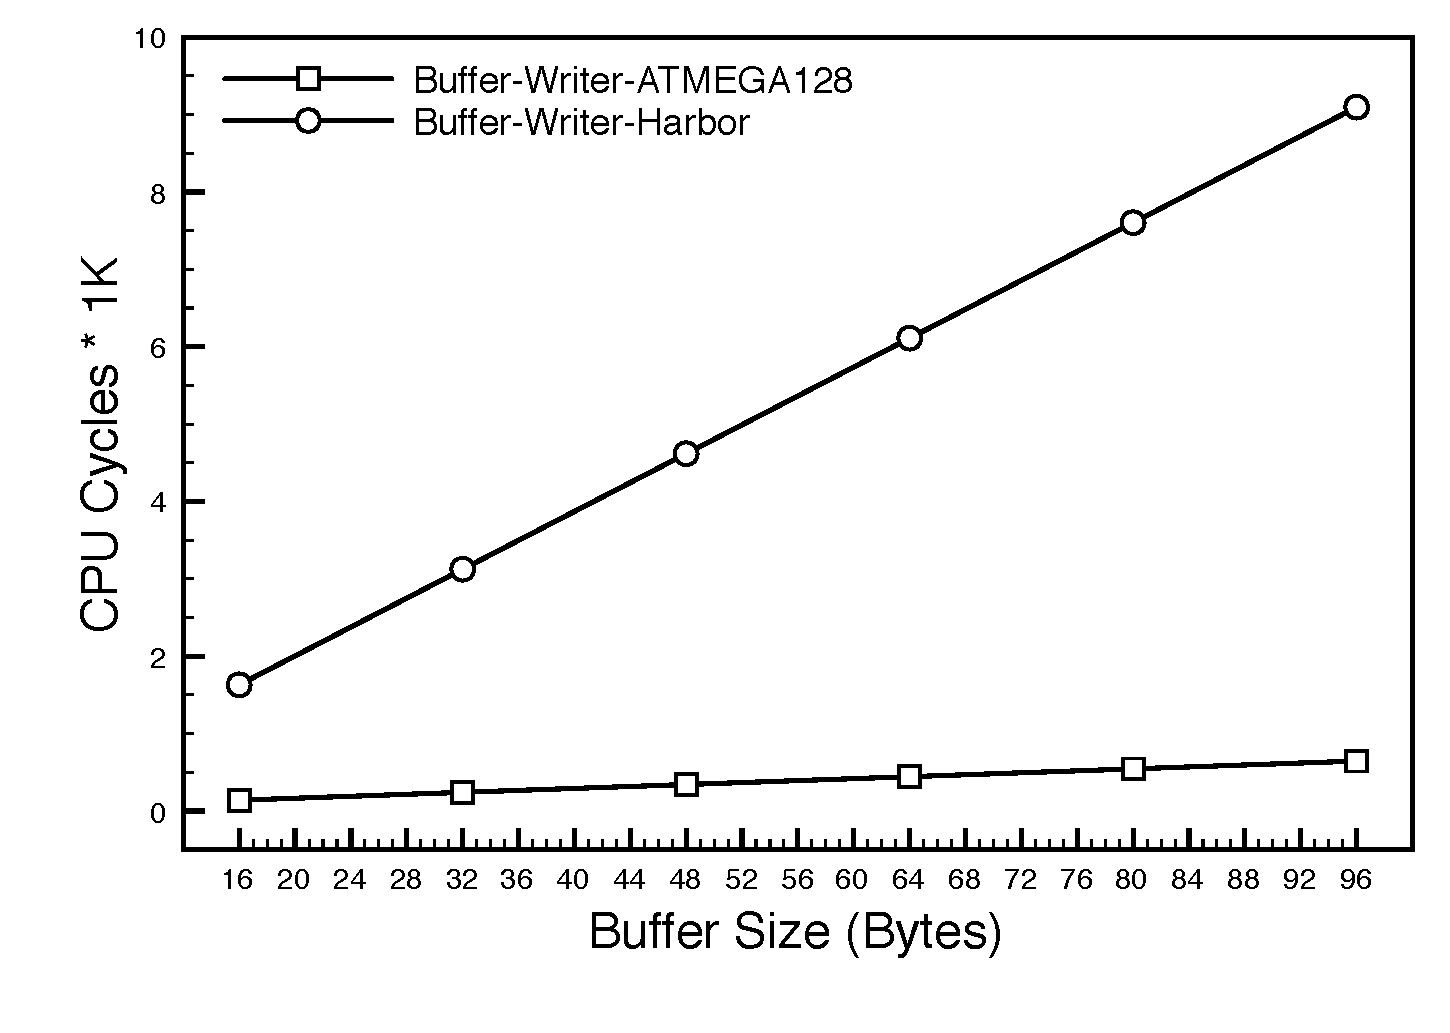
\includegraphics[width=1.8in,
      keepaspectratio = true]{figures/bufferwriterharbor.eps}}
    \hspace{0.05in}
    \subfigure[DVM Overhead]{\label{fig:bffwrdvm}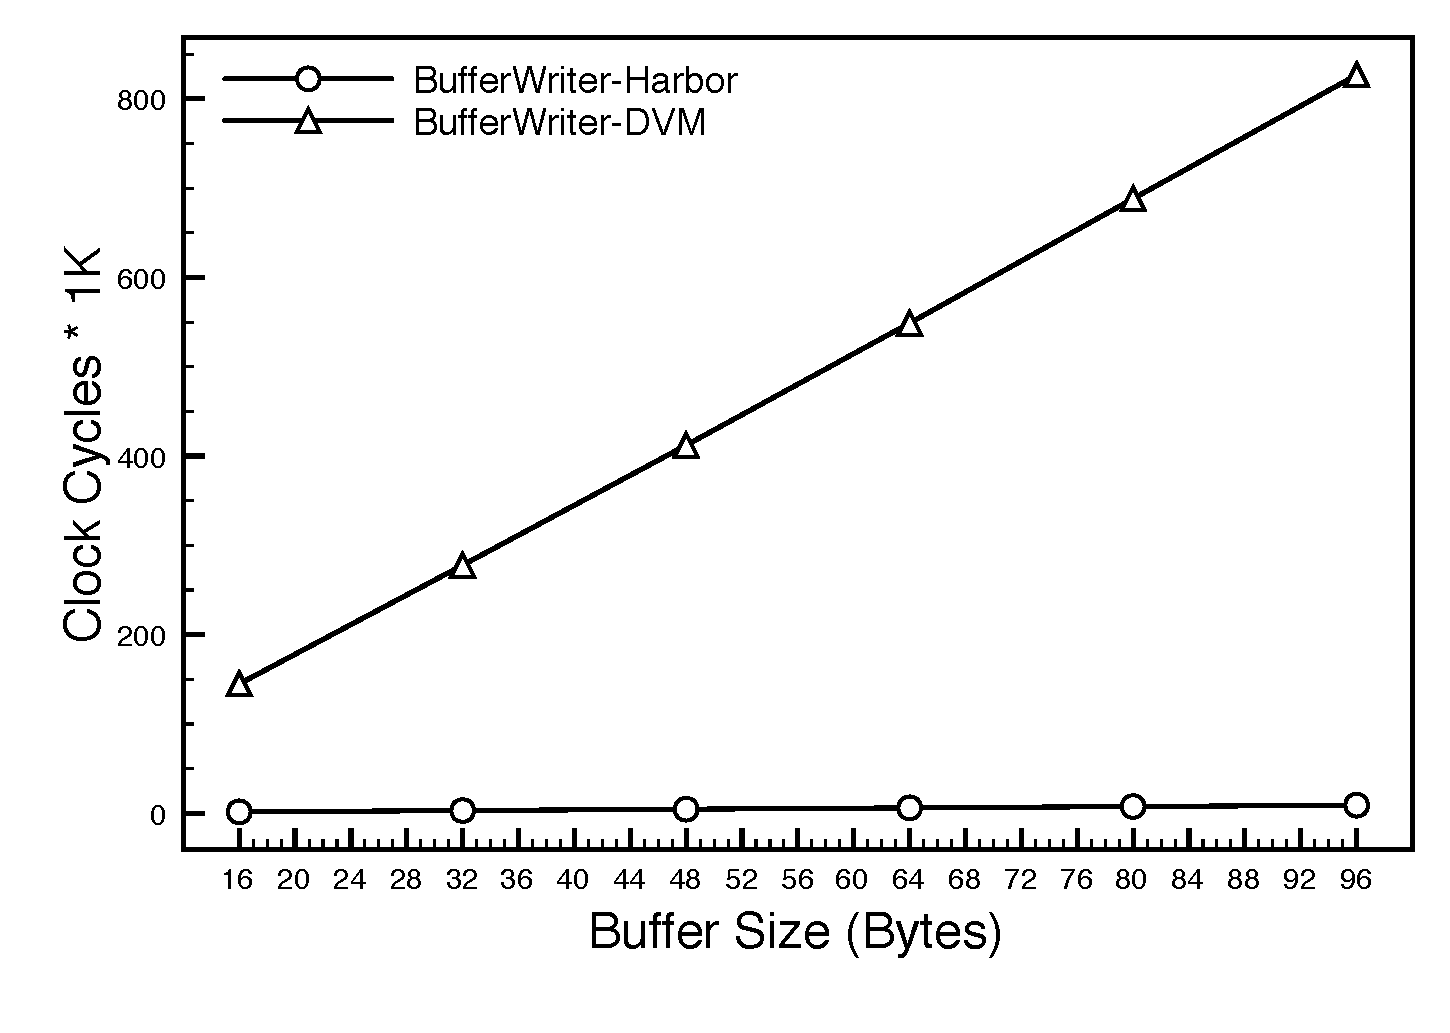
\includegraphics[width=1.8in,
      keepaspectratio = true]{figures/bufferwriterdvm.eps}}
    \hspace{0.05in}
    \subfigure[UMPU Overhead]{\label{fig:bffwrumpu}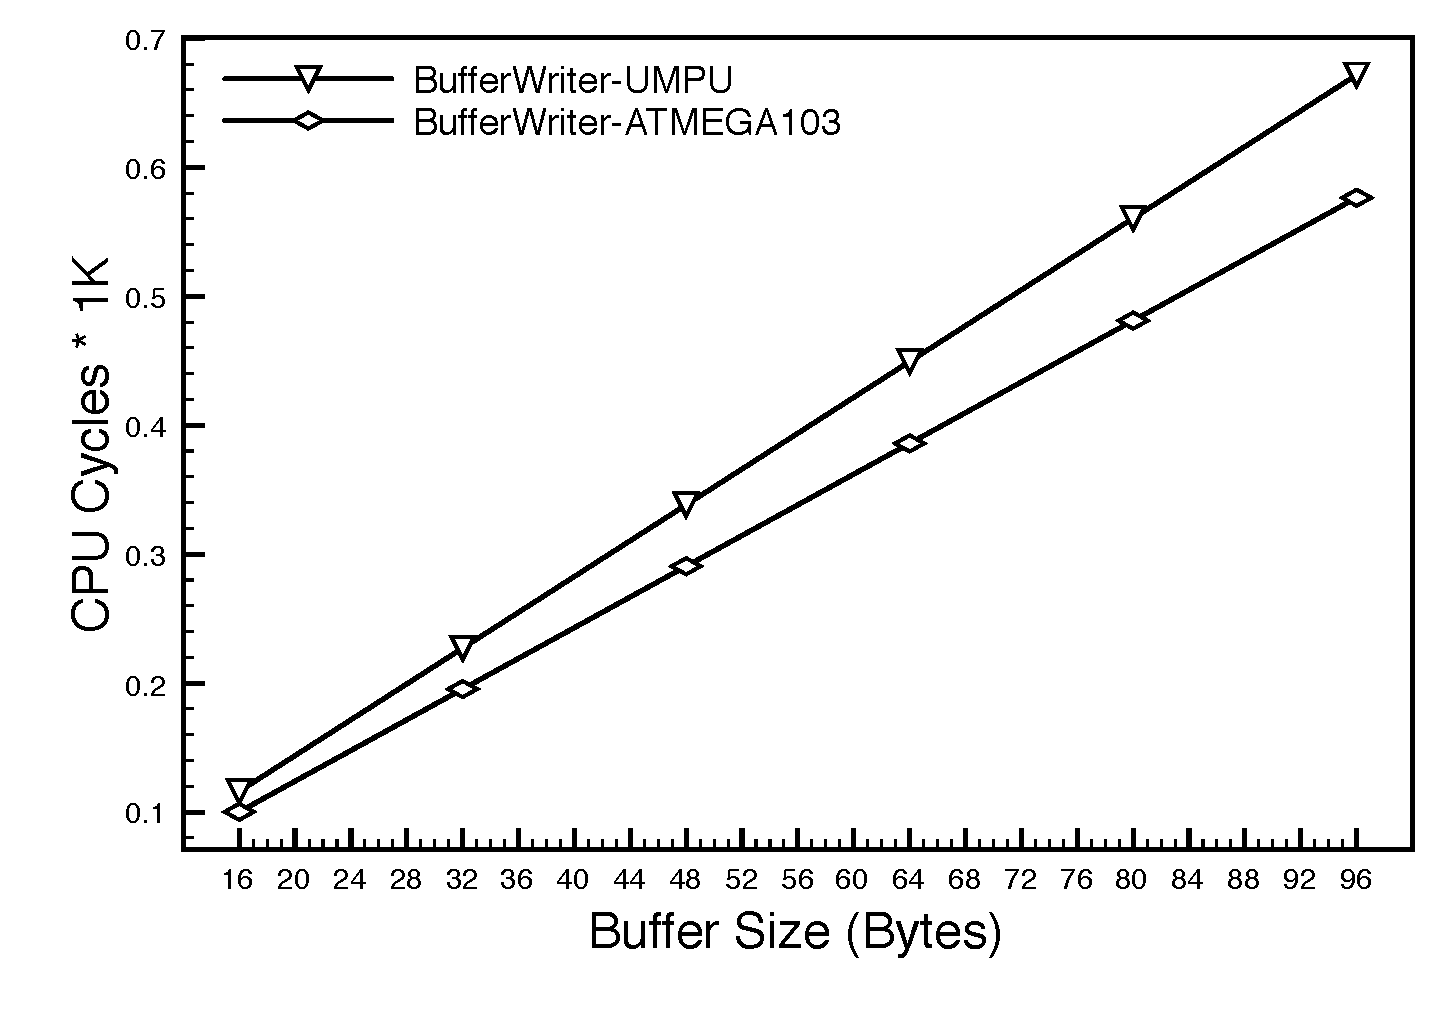
\includegraphics[width=1.8in,
      keepaspectratio = true]{figures/bufferwriterumpu.eps}}
  }
  \label{fig:buff_writer}
  \caption{Buffer Writer Performance}
\end{figure}   

%----------------------------------------
\subsubsection{Data Collector}
%
We next consider a typical duty-cycled sensor network application,
namely data gathering through a collection tree.
%
Our experiment setup was a simulated network of 5 Mica2 motes arranged
in a linear topology to form a two-hop network to a base station.
%
All nodes were installed with an SOS kernel with 8-domain Harbor protection.
%
When the network was up, the two-module data collection application was
installed on all nodes.
%
First, a tree building and maintenance module~\cite{woo03surge} was
distributed; then
%
the Surge module, which periodically samples light sensor data and sends it
to the base station via the collection tree, was installed.
%
The two modules were installed in different protection domains.
%
Harbor's impact on the complete application was measured by profiling CPU
active time in the Avrora simulator.
%
CPU active time was observed to be 8.41\% and 8.56\% over a duration
of 30 minutes for normal and protected mode operation, respectively. 
%
The relative increase in CPU utilization for a protected system is
thus only 1.85\% compared to an unprotected system.
%
In most sensor network applications, absolute CPU utilization is even
lower~\cite{tkernel06sensys}.
%
The increased overhead is a small price to pay for the improved
reliability provided by the software-based memory protection.
%----------------------------------------
\subsubsection{SOS Serial Stack}
%
Sensor network software needs to respond to events occurring in the
physical environment.
%
Efficient interrupt handling is critical to ensure a reactive system.
%
In this subsection, we evaluate the performance impact of memory
protection on the serial driver's interrupt service routine.
%
We isolate the Serial Stack from the SOS kernel and install it in a
separate protection domain.
%
The Serial Stack in SOS is a complex system comprising of multiple
layers (shown in Figure~\ref{fig:serialstack}) that implements the
High-Level Data Link Control (HDLC) protocol for communication between
a pair of nodes.
%
\begin{figure}[htbp]
  \centering
   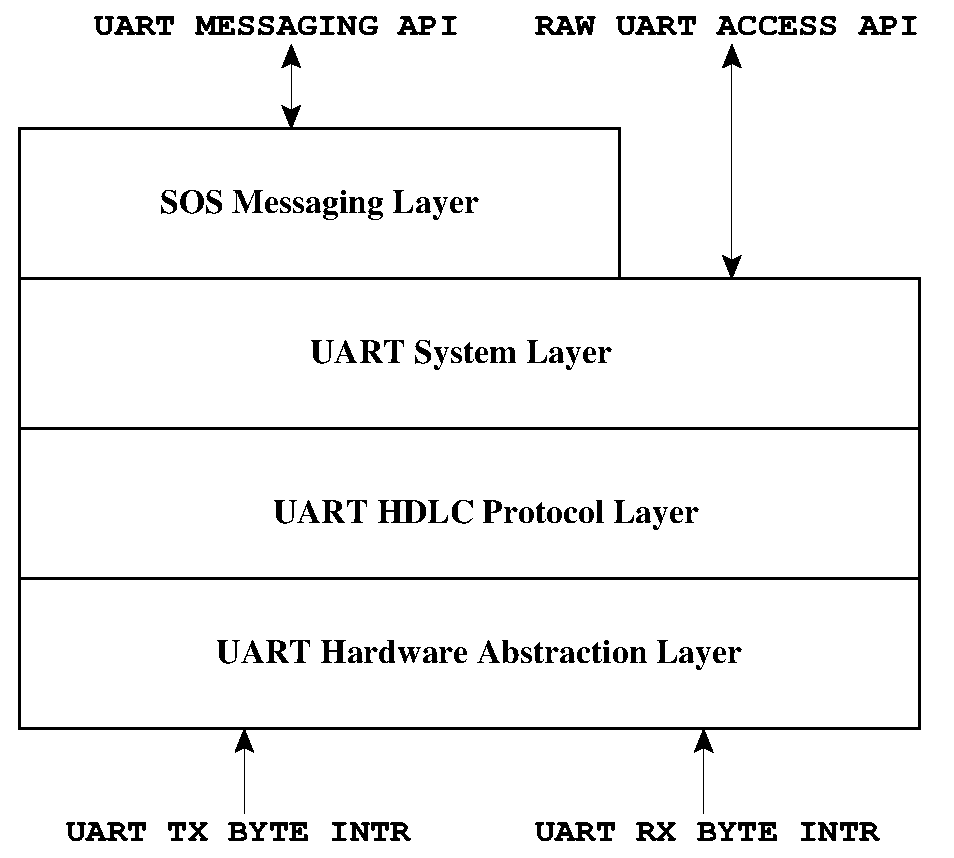
\includegraphics[height = 1.5in,
   keepaspectratio=true]{figures/serialstack.eps} 
   \caption{SOS Serial Stack Layers}
   \label{fig:serialstack}
\end{figure}
%

Our experiment set up consists of a sensor node simulated in Modelsim
with UMPU enabled.
%
An application periodically sends a SOS message outside the
sensor node through the serial port.
%
The transmitted message is echoed back to the sensor node and is
received by the application.
%
The UART hardware and the serial stack is capable of full-duplex
operation.
%
All the processing in the serial stack occurs within the send and
receive interrupts.
%
%
\begin{figure}[htpb]
  \label{fig:intrtrace}
  \centering
  \mbox{
    \subfigure[Rx Interrupt Latency]{\label{fig:rxintr}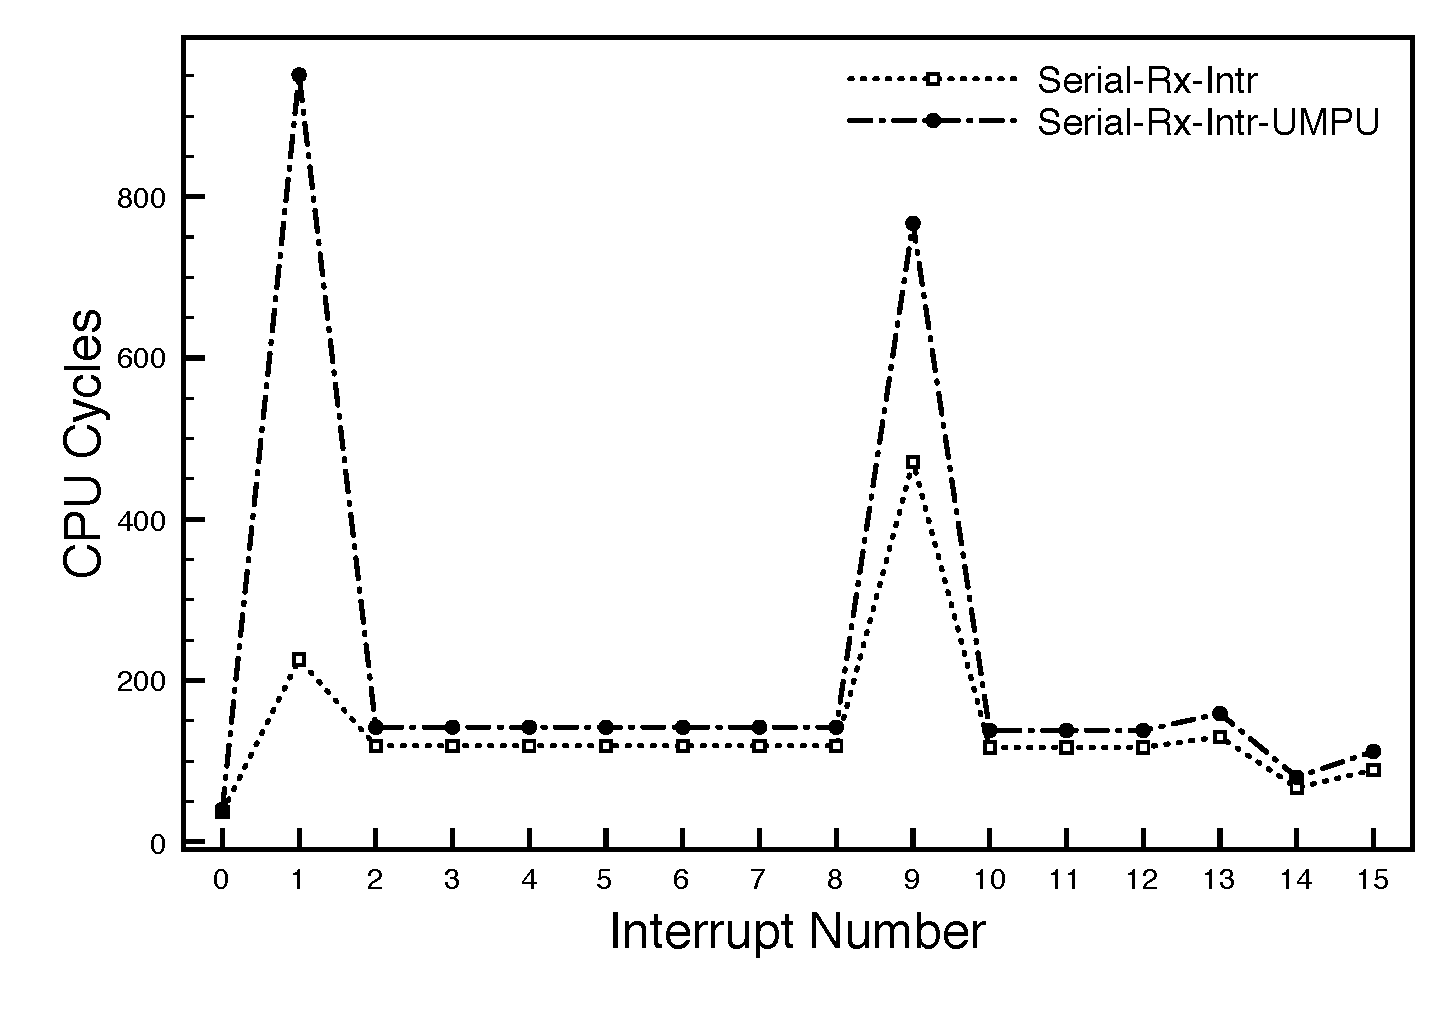
\includegraphics[width=2.5in,
      keepaspectratio = true]{figures/rxintr.eps}}
    \hspace{0.2in}
    \subfigure[Tx Interrupt Latency]{\label{fig:txintr}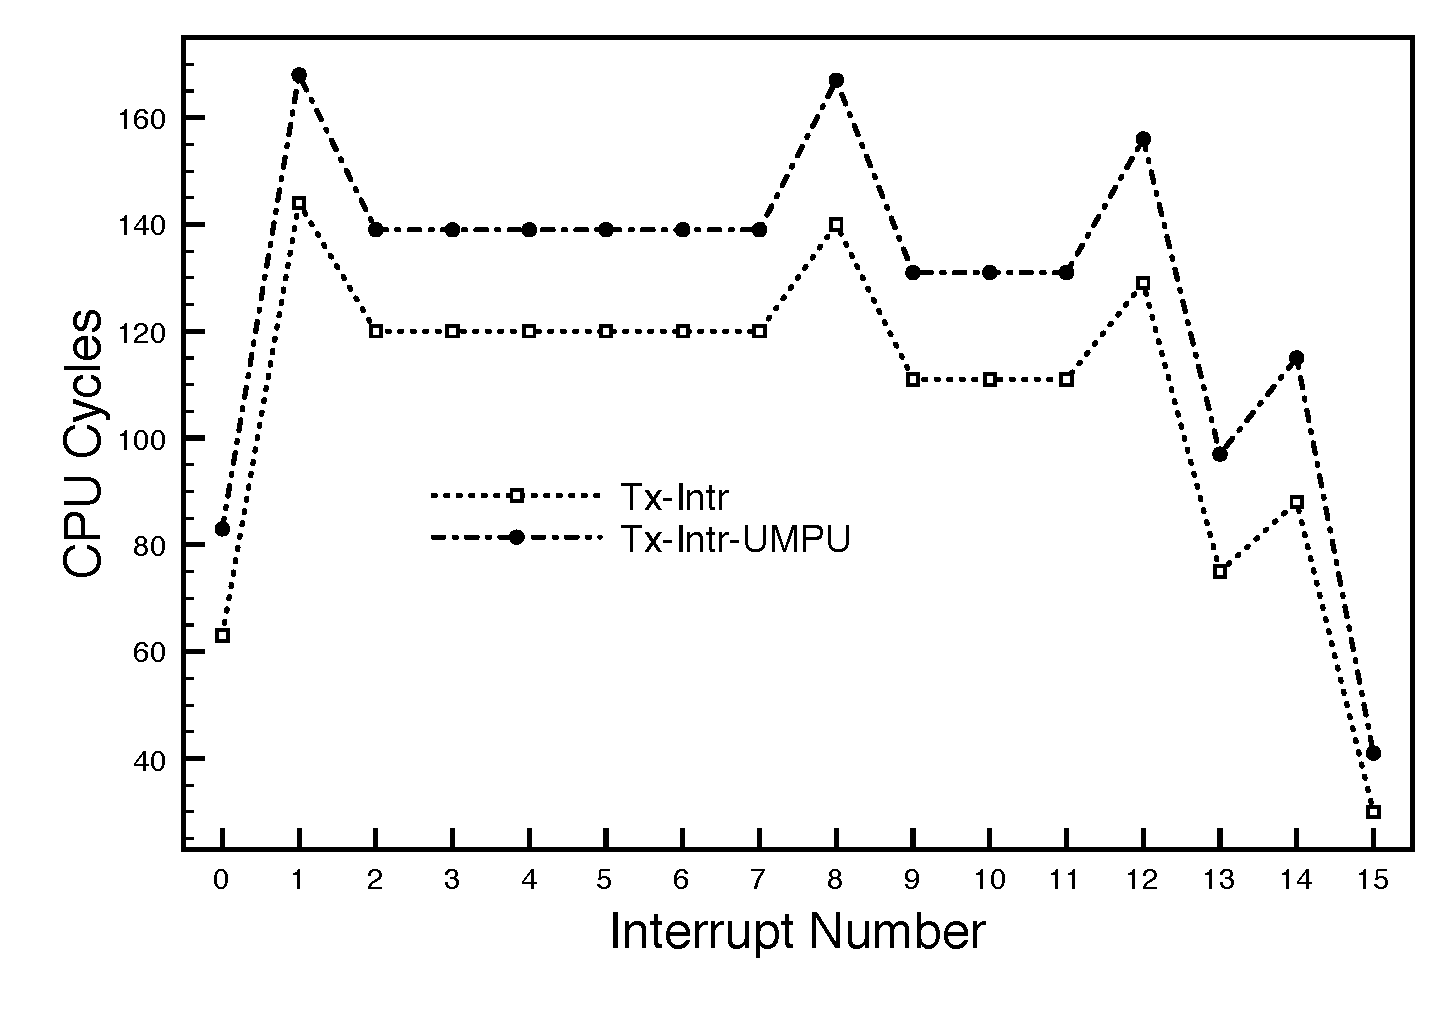
\includegraphics[width=2.5in,
      keepaspectratio = true]{figures/txintr.eps}}
  }
  \caption{Serial Stack Execution Trace}
\end{figure}   
%

Figure~\ref{fig:rxintr} contains a trace of the receive interrupt
service time with the protection enabled and disabled.
%
The execution time with UMPU enabled has a constant overhead of 23 clock
cycles except for interrupt number 1 and 9.
%
In the current UMPU implementation, all the interrupts originate in
the trusted domain and the control is transferred to the real
interrupt handler through a cross domain call.
%
The cross domain call through the jump table takes 13 clock cycles,
the corresponding cross domain return takes 9 clock cycles and the
execution of the interrupt handler takes one extra clock cycle to
check the memory map before storing the received byte.
%

Interrupt 1 allocates a SOS message data structure to store the
received message.
%
The UMPU disabled serial driver implementation allocates the message
from a pre-allocated pool of messages.
%
However, the UMPU enabled serial driver implementation cannot
pre-allocate a message pool as the memory map cannot track ownership
of data structures within an allocated segment.
%
This is a limitation of the memory map design.
%
Therefore, UMPU enabled serial driver has to incur the significantly
higher cost of memory allocation.
%

Interrupt 9 allocates the payload for the received message.
%
The higher latency of the UMPU enabled serial driver is due to the
higher overhead of memory allocation routines in the UMPU software
library.
%

The trace of the Transmit interrupt service time (Figure~\ref{fig:txintr}) shows only a constant
overhead caused due to the cross domain call mechanisms.
%
This experiment demonstrates that the protection benefits of UMPU can
be obtained without any loss in the performance of latency sensitive
routines.
%
%================================================================
% RESILIENCE TO APPLICATION FAULTS
%================================================================
\subsection{Experience} 
%
Harbor has been in use in SOS for several months, and has
%
discovered two memory corruption faults in application modules that had
been in active use for several months previously.
%
The first error was discovered while executing the data collection
application on a SOS kernel with 2-domain Harbor protection.
%
A programming error in the Surge module triggered an invalid memory access exception.
%
Figure~\ref{fig:surge_error} demonstrates the error.

\begin{figure} [h]
  \centering
\begin{small}
\begin{verbatim}
     // Size of routing header
     hdr_size = SOS_CALL(s->get_hdr_size, proto);
     // Using return value without checking 
     s->smsg = (SurgeMsg*)(pkt + hdr_size); 
     // Memory Corruption
     s->smsg->type = SURGE_TYPE_SENSORREADING;  
\end{verbatim} 
\vskip-\baselineskip
\end{small}
  \caption{Programming error in Surge module}
  \label{fig:surge_error}
\end{figure}

\noindent
%
The Surge module invokes a dynamic function call~\cite{ram05sos} to
the tree routing module to determine the size of the routing header.
%
Dynamic function calls are linked at run time, and fail with an error
code if the function provider is absent.
%
The code above fails to check whether \verb+hdr_size+ is an error code.
%
Nodes where the Surge module was installed before the tree routing module
would use an negative value for the routing header size and thereby corrupt
memory---specifically, heap metadata, which effectively resides in the
kernel domain.
%
Harbor detected this error and killed the offending application.


%
A second programming error was discovered in the tree routing module with
8-domain protection.
%
There were three active domains in the system: the kernel, the tree routing
module, and the buffer writer module.
%
The SOS kernel tracks the ownership of a message payload as it is passed from a source module to its destination module.
%
If the source module wishes to relinquish ownership, it sets a release flag while posting the message.
%
A destination module that wishes to write into the message payload is
\emph{required} to gain ownership through a \verb+sys_msg_take_data+ system
call.  If the source module set the release flag, this system call is
effectively a no-op.  If the source module did not set the flag, however,
then the system call makes a private copy of the payload owned by the
destination module.
%
Failure to call \verb+sys_msg_take_data+ could corrupt the source module's
memory.
%
The buffer writer module was not releasing the buffer, but the tree routing
module was not calling \verb+sys_msg_take_data+.
%
Harbor discovered this error when the tree routing module tried to
overwrite the message payload.
%

The errors described in this section occur under rare conditions and
are hard to detect during software testing.
%
However, the impact of these errors could be severe.
%
A system that can guarantee memory protection is indispensable for
building robust embedded software.























%===========================================================================
% CONCLUSION
%===========================================================================
\section{Conclusion}
\label{sec:conclude}
%
In this paper, we have proposed a hardware software co-design approach for providing memory protection in tiny embedded processors.
%
Though we have implemented the protection technology for the AVR microcontroller, our general approach is applicable to other RISC architectures such as TI MSP or ARM.
%
Through a careful partitioning of the protection techniques, we have significantly improved performance by moving compute intensive operations into hardware.
%
Our hardware is very flexible, it can accommodate various configuration parameters.
%
The software library provides a standard programming interface.
%
Moreover, our approach does not modify the instruction set architecture of the processor; hence we do not need to modify the cross compiler.
%
These features ensure that our software library can be incorporated into existing projects with minimal modifications; a very practical benefit to the system developers.
%
We are still exploring the design space of possible protection architectures.
%
The resource utilization of our design can be further reduced by synthesizing hardware units that are pre-configured for a particular block size and number of protection domains.
%
An interesting area of future work is to explore software techniques such as virtual machines or type-safe languages  that can benefit from modest hardware extensions.
%
Software reliability is an emerging concern in the domain of tiny embedded processors.
%
Limited resources preclude the application of existing approaches used in desktop processors.
%
We believe that hardware software co-design techniques are a promising avenue to explore for creating robust software for tiny embedded processors. 



\bibliographystyle{unsrt}
\bibliography{harbor-tecs}


\begin{received}
...
\end{received}
\end{document}


